\chapter{Projekt: mapy náhodných ostrovov}
\label{sect:ostrovy}

Náhodné čísla majú veľa rôznych použití. Môžu pomôcť niečo efektívnejšie naprogramovať,
ako sme videli pri porovnávaní súborov. Môžu sa s nimi vyrábať testovacie vstupy 
pri ladení programov. A dajú sa dobre využiť aj pri generovaní rôznych vecí,
ktoré chceme, aby zakaždým vyzerali inak. Tu sa hodí, že máme pseudonádondé
čísla: na rozdiel od náhodných totiž môžeme použiť seed na to, aby sme
``náhodné'' veci presne zopakovali, ak treba. Určite poznáš rôzne hry, ktoré
vedia generovať náhodné svety. Predpokladajme,
že dej hry sa odohráva na hornatom ostrove 
a chceme, aby sa zakaždým vygeneroval iný. 
V tomto projekte chceme vygenerovať náhodný ostrov a vykresliť ho v štýle starých 
tieňovaných máp nejak takto:

\vskip 3ex
\centerline{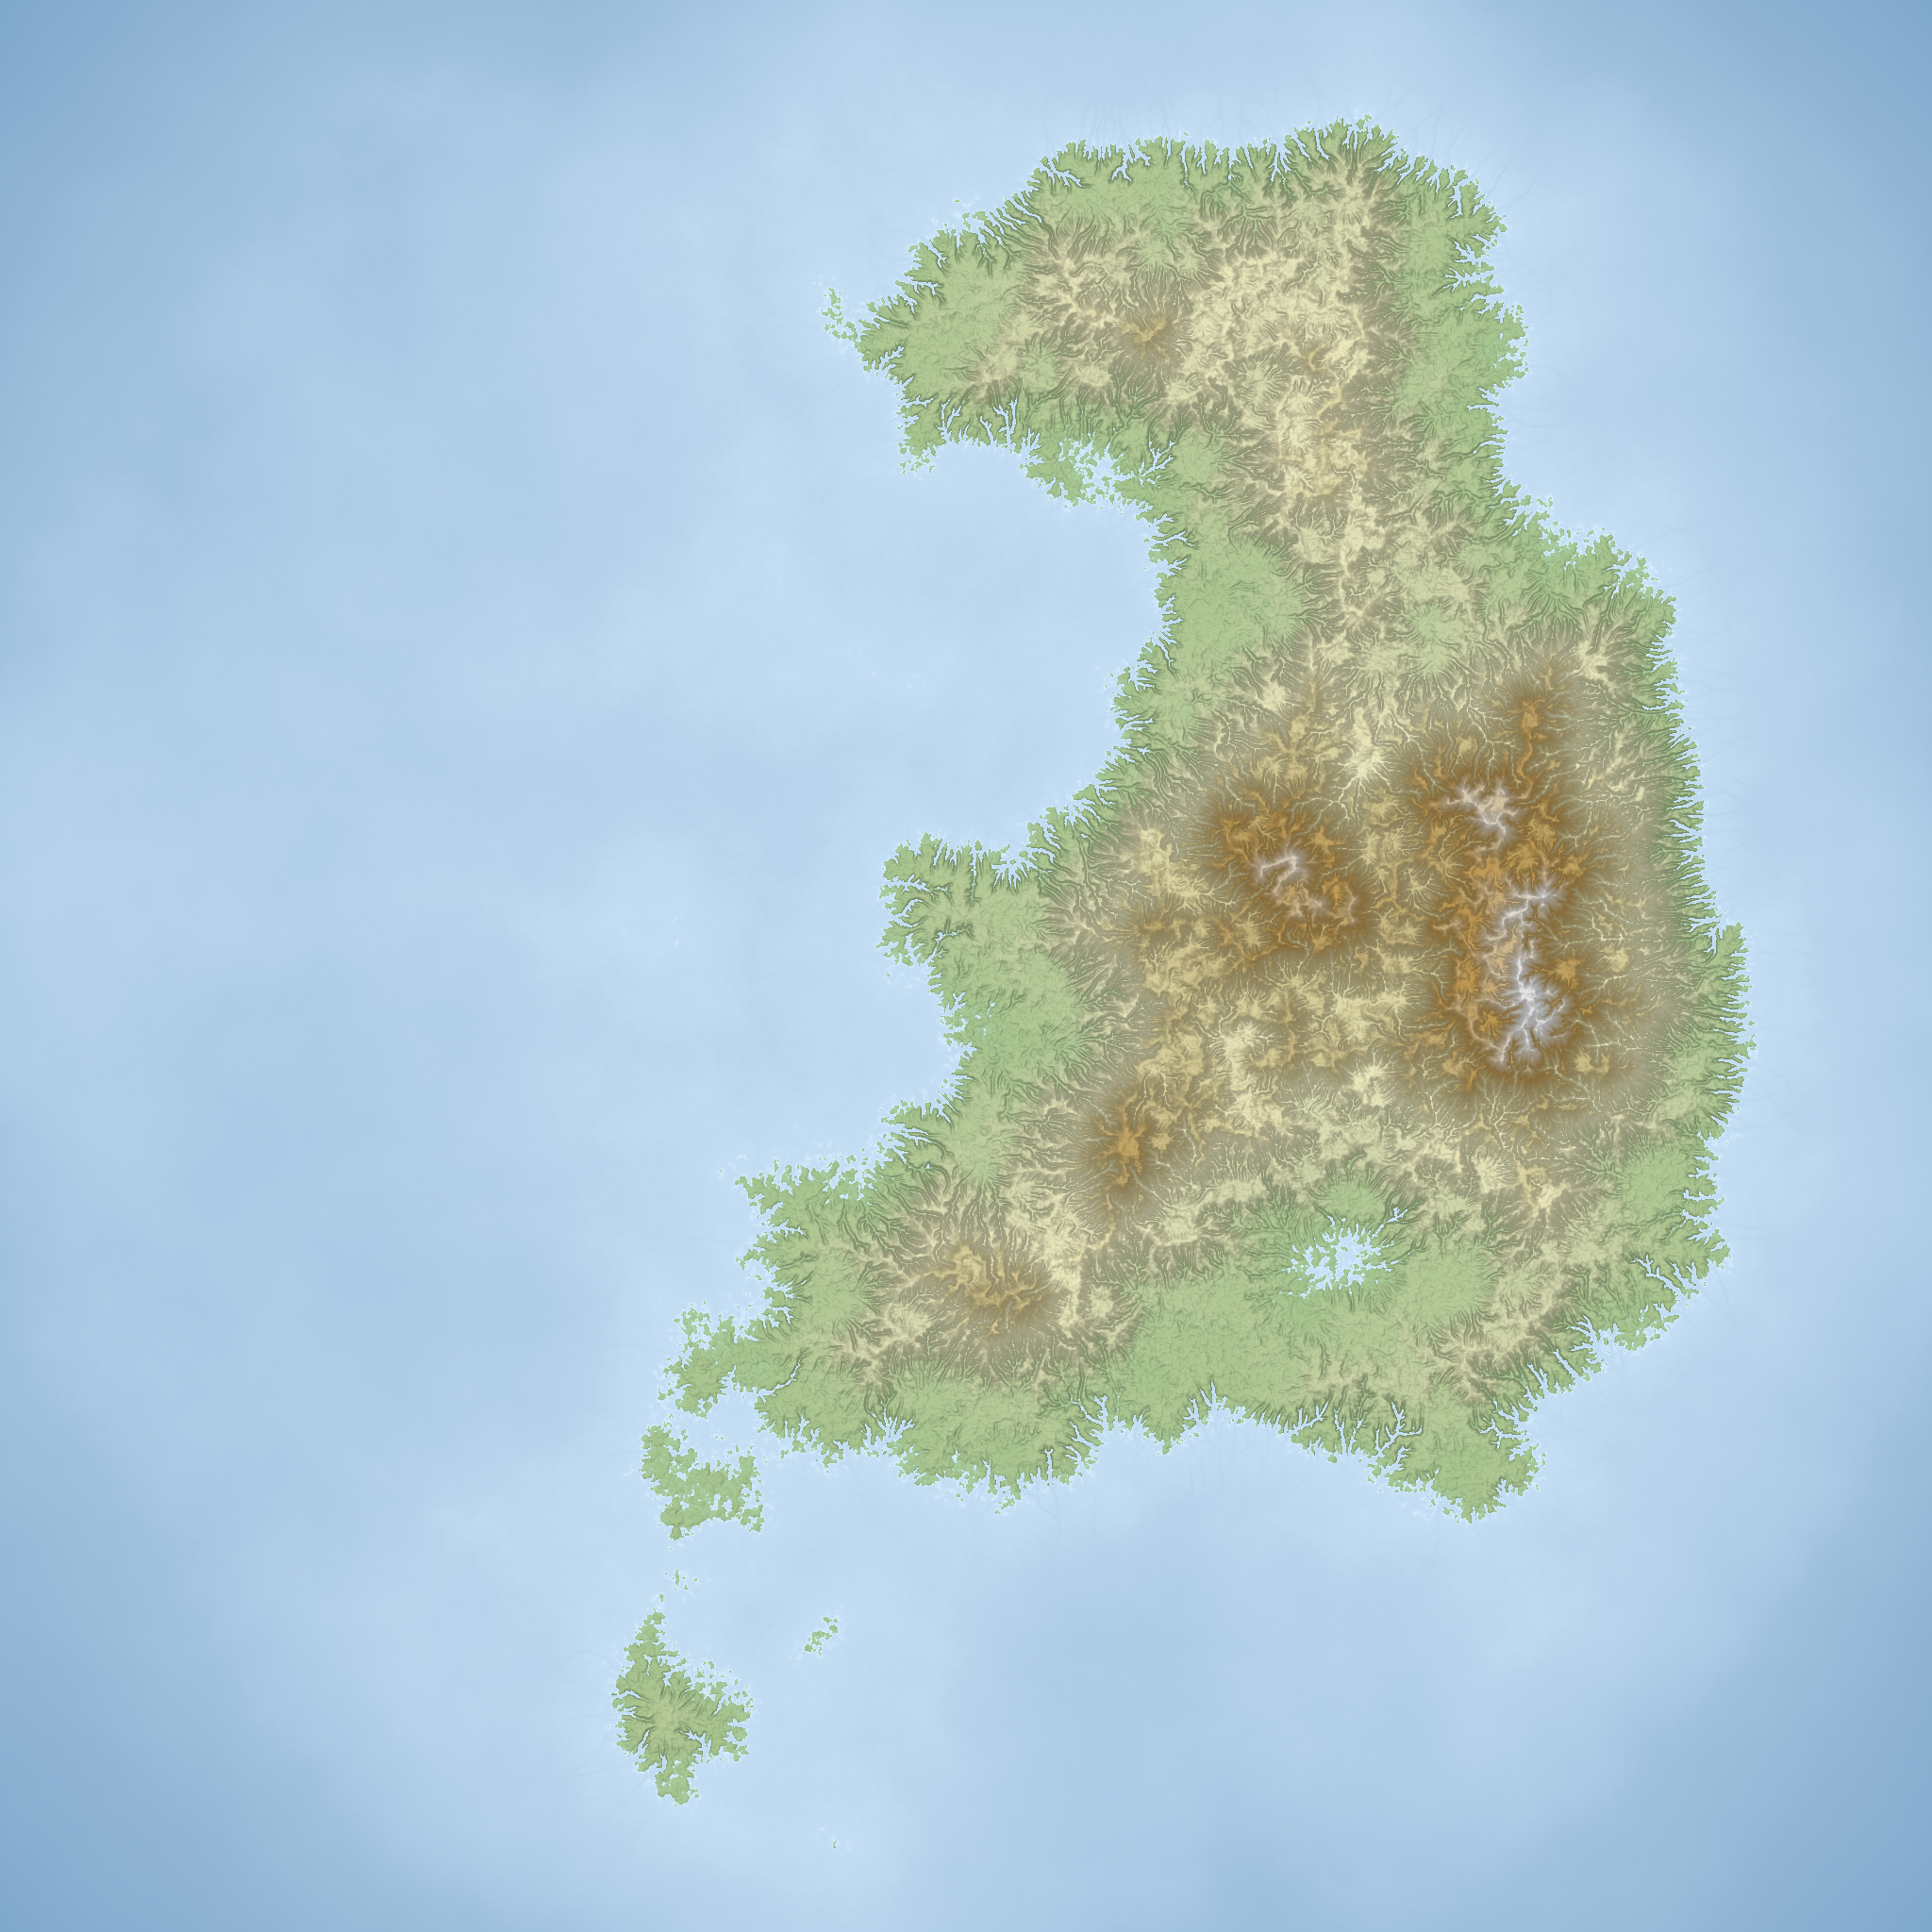
\includegraphics[width=0.9\textwidth]{data/86_rendered.png}}
\vskip 3ex

Úlohu si rozdelíme na menšíe časti a o každej z nich si niečo povieme.
Najprv si  vyrobíme 
výškovú mapu ({\em heightmap}): tabuľku \prg!double! s číslami z rozsahu\indexItem{Alg}{výšková mapa}
$0\ldots1$, kde $0$ znamená najmenšiu a $1$ najväčšiu výšku (obrázok A).
Z nej potom urobíme dva obrázky: jeden, ktorý bude určovať farbu získame tak,
že každému pixelu priradíme farbu z nejakého gradientu podľa jeho výšky (obrázok B)
a druhý, ktorý bude určovať tiene, vyrobíme  podľa sklonu terénu (obrázok C). Napokon
oba obrázky spojíme do výsledku (obrázok D).



\centerline{
  \begin{tikzpicture}[scale=5]
    \def\tmp#1{\includegraphics[width=3.8cm]{data/86_#1.png}}
    \node (A) at (0,0) {\tmp{heightmap}};
    \node (B) at (1,0) {\tmp{colored}};
    \node (D) at (2,0) {\tmp{rendered}};
    \node (C) at (1,-1) {\tmp{normal}};

    \foreach \a in {A,B,C,D}
    \node [above = of \a, yshift = -11mm] {(\a)};

    \draw[->] (A) -- (B);
    \draw[->] (B) -- (D);
    \draw[->] (A) to[out=270,in=180] (C);
    \draw[->] (C) to[out=0,in=270] (D);
  \end{tikzpicture}}

Začneme s prípravnou prácou: na zapisovanie finálneho výsledku môžeme použiť náš starý súbor
\hbox{\link{\rootpath/obrazok.h}{obrazok.h}.} Okrem toho budeme veľa robiť s tabuľkami,
kde budeme mať buď reálne čísla alebo farby, tak je dobré sa na to pripraviť.

\begin{uloha}
  Uprav triedu \vb{Tabulka} z kapitoly \ref{sect:cukor} tak, aby sa v nej 
  dali ukladať akékoľvek typy (pomocou šablóny).
\end{uloha}

Prvý pokus o náhodnú výškovú mapu môže vyzerať nejak takto\footnote{\indexItem{Prg}{inkrement \vb{i++} ako výraz}%
Tu idem použiť zápis, ktorý sme doteraz nemali a zaslúži si komentár. Ak mám napr. premennú
\prg!int i!, tak vieš, že \prg!i++! je príkaz, ktorý priráta k \prg!i! jednotku. Doteraz som ti
nepovedal, že \prg!i++! sa dá použiť aj ako výraz. Keby som mal napr. \prg!vector<int> a!,
tak \prg!int x = a[i++]! znamená \cmd{Do \prg!x! ulož hodnotu \prg!a[i]! a potom zvýš \prg!i! o jednotku}.
Je to teda to isté, ako keby som napísal \prg!x = a[i]; i = i+1;!.
Niekedy si možno zbadal aj zápis \prg!++i!, ktorý sám osebe robí to isté, t.j. pripočíta k \prg!i! jednotku,
ale urobí to na začiatku. Preto \prg!int y = a[++i]! je to isté ako \prg!i = i+1; y = a[i];!
}

\begin{lstlisting}
#include <algorithm>
#include <fstream>
#include <iostream>
#include <random>
#include <sstream>
#include <vector>

#include "obrazok.h"
#include "tabulka.h"

using namespace std;
mt19937 rnd(random_device{}());
uniform_real_distribution<> dis(0.0, 1.0);

void zapis(Tabulka<double>& T, const char* fname) {
  vector<unsigned char> data(T.m * T.n * 4);
  for (int i = 0; i < T.m; i++)
    for (int j = 0; j < T.n; j++) {
      int offs = 4 * ((T.n - j - 1) * T.n + i);
      for (int k = 0; k < 3; k++)
        // min a max sú z knižnice <algorithm> a vrátia menšie a väčšie z dvojice čísel
        data[offs++] = min(255 * max(T(i, j), 0.0), 255.0);
      data[offs++] = 255;
    }
  zapis_rgba_png(T.n, T.m, data.data(), fname);
}

int main(int argc, char** argv) {
  if (argc > 1) {
    unsigned long seed;
    stringstream ss(argv[1]);
    ss >> seed;
    rnd.seed(seed);
  }
  int n = 1024;
  Tabulka<double> T(n, n);
  for (int i = 0; i < n; i++)
    for (int j = 0; j < n; j++) T(i, j) = dis(rnd);

  zapis(T, "sum.png");
}
\end{lstlisting}


V tomto programe som si spravil pomocnú funkciu
\vb{zapis()}, ktorá zoberie tabuľku s výškovou mapou
a zapíše z nej obrázok do súboru tak, že nula je čierna a jednotka je biela. Pri zapisovaní 
obrázka potrebujem na jeden pixel štyri byty \vb{r,g,b,a}. Keďže chcem vyrobiť odtiene sivej,
hodnoty \vb{r,g,b} nastavím všetky rovnako, a to na hodnotu \vb{255 * T(i,j)}.

 
V hlavnom si vyrobím náhodný generátor a pozriem sa,  či nie je na príkazovom riadku parameter. Ak je, zoberiem ho ako seed. Ak budem 
chcieť zopakovať ten istý ostrov, stačí zadať rovnaký seed. Spustím program a výsledok je



\centerline{\begin{tikzpicture}[scale=0.8]

  \coordinate (A) at (-2mm,-2mm);
  \coordinate (B) at (4cm, 1cm);
  \draw[red] (A) -- (B);
  \filldraw[draw=red, fill=white] (A) circle (1mm) (B) circle (2.5cm);

  \node[anchor=north east] at (0,0) {
\includegraphics[width=6cm]{data/sum.png}};
  \node at (B) {
\includegraphics[width=2.6cm]{data/sum_big.png}};
  \draw[draw=red] (A) circle (1mm) (B) circle (2.5cm);
\end{tikzpicture}}


Ugh. Zväčšený roh vpravo ukazuje, prečo to nefunguje: keďže každý pixel je 
nezávislé náhodné číslo, nie je medzi nimi žiaden vzťah. Hodnoty medzi jednotlivými
pixelmi skáču tak, že výsledkom, keď sa naňho pozerám trochu z diaľky, je sivá plocha.
Potrebujem niečo, čo by síce bolo náhodné, ale zasa nie až tak úplne. Ukážem ti 
jednu z možností, ako náhodnosť regulovať. Volá sa podľa chlapíka, čo s tým prvý prišiel,\indexItem{Alg}{Perlin noise}
{\em Perlin noise}. S ním sa dajú generovať rôzne veľké náhodné vzory, ktorých kombináciou
vznikajú fraktálovité náhodné útvary.\\


% perlin 17
\centerline{\begin{tikzpicture}[scale=3.4]
  \foreach \i in {0,1} {
    \foreach \j in {0,1,2} {
      \pgfmathtruncatemacro{\tmp}{1+3*\i+\j}
      \node at (\j,-\i) {\includegraphics[width=31mm]{data/sample_perlin_\tmp.png}};
      }}

  \node[draw, single arrow, minimum height=12mm, minimum width=8mm,
  single arrow head extend=2mm, anchor=center] at (2.75,-0.5) {};

      \node at (3.5,-0.5) {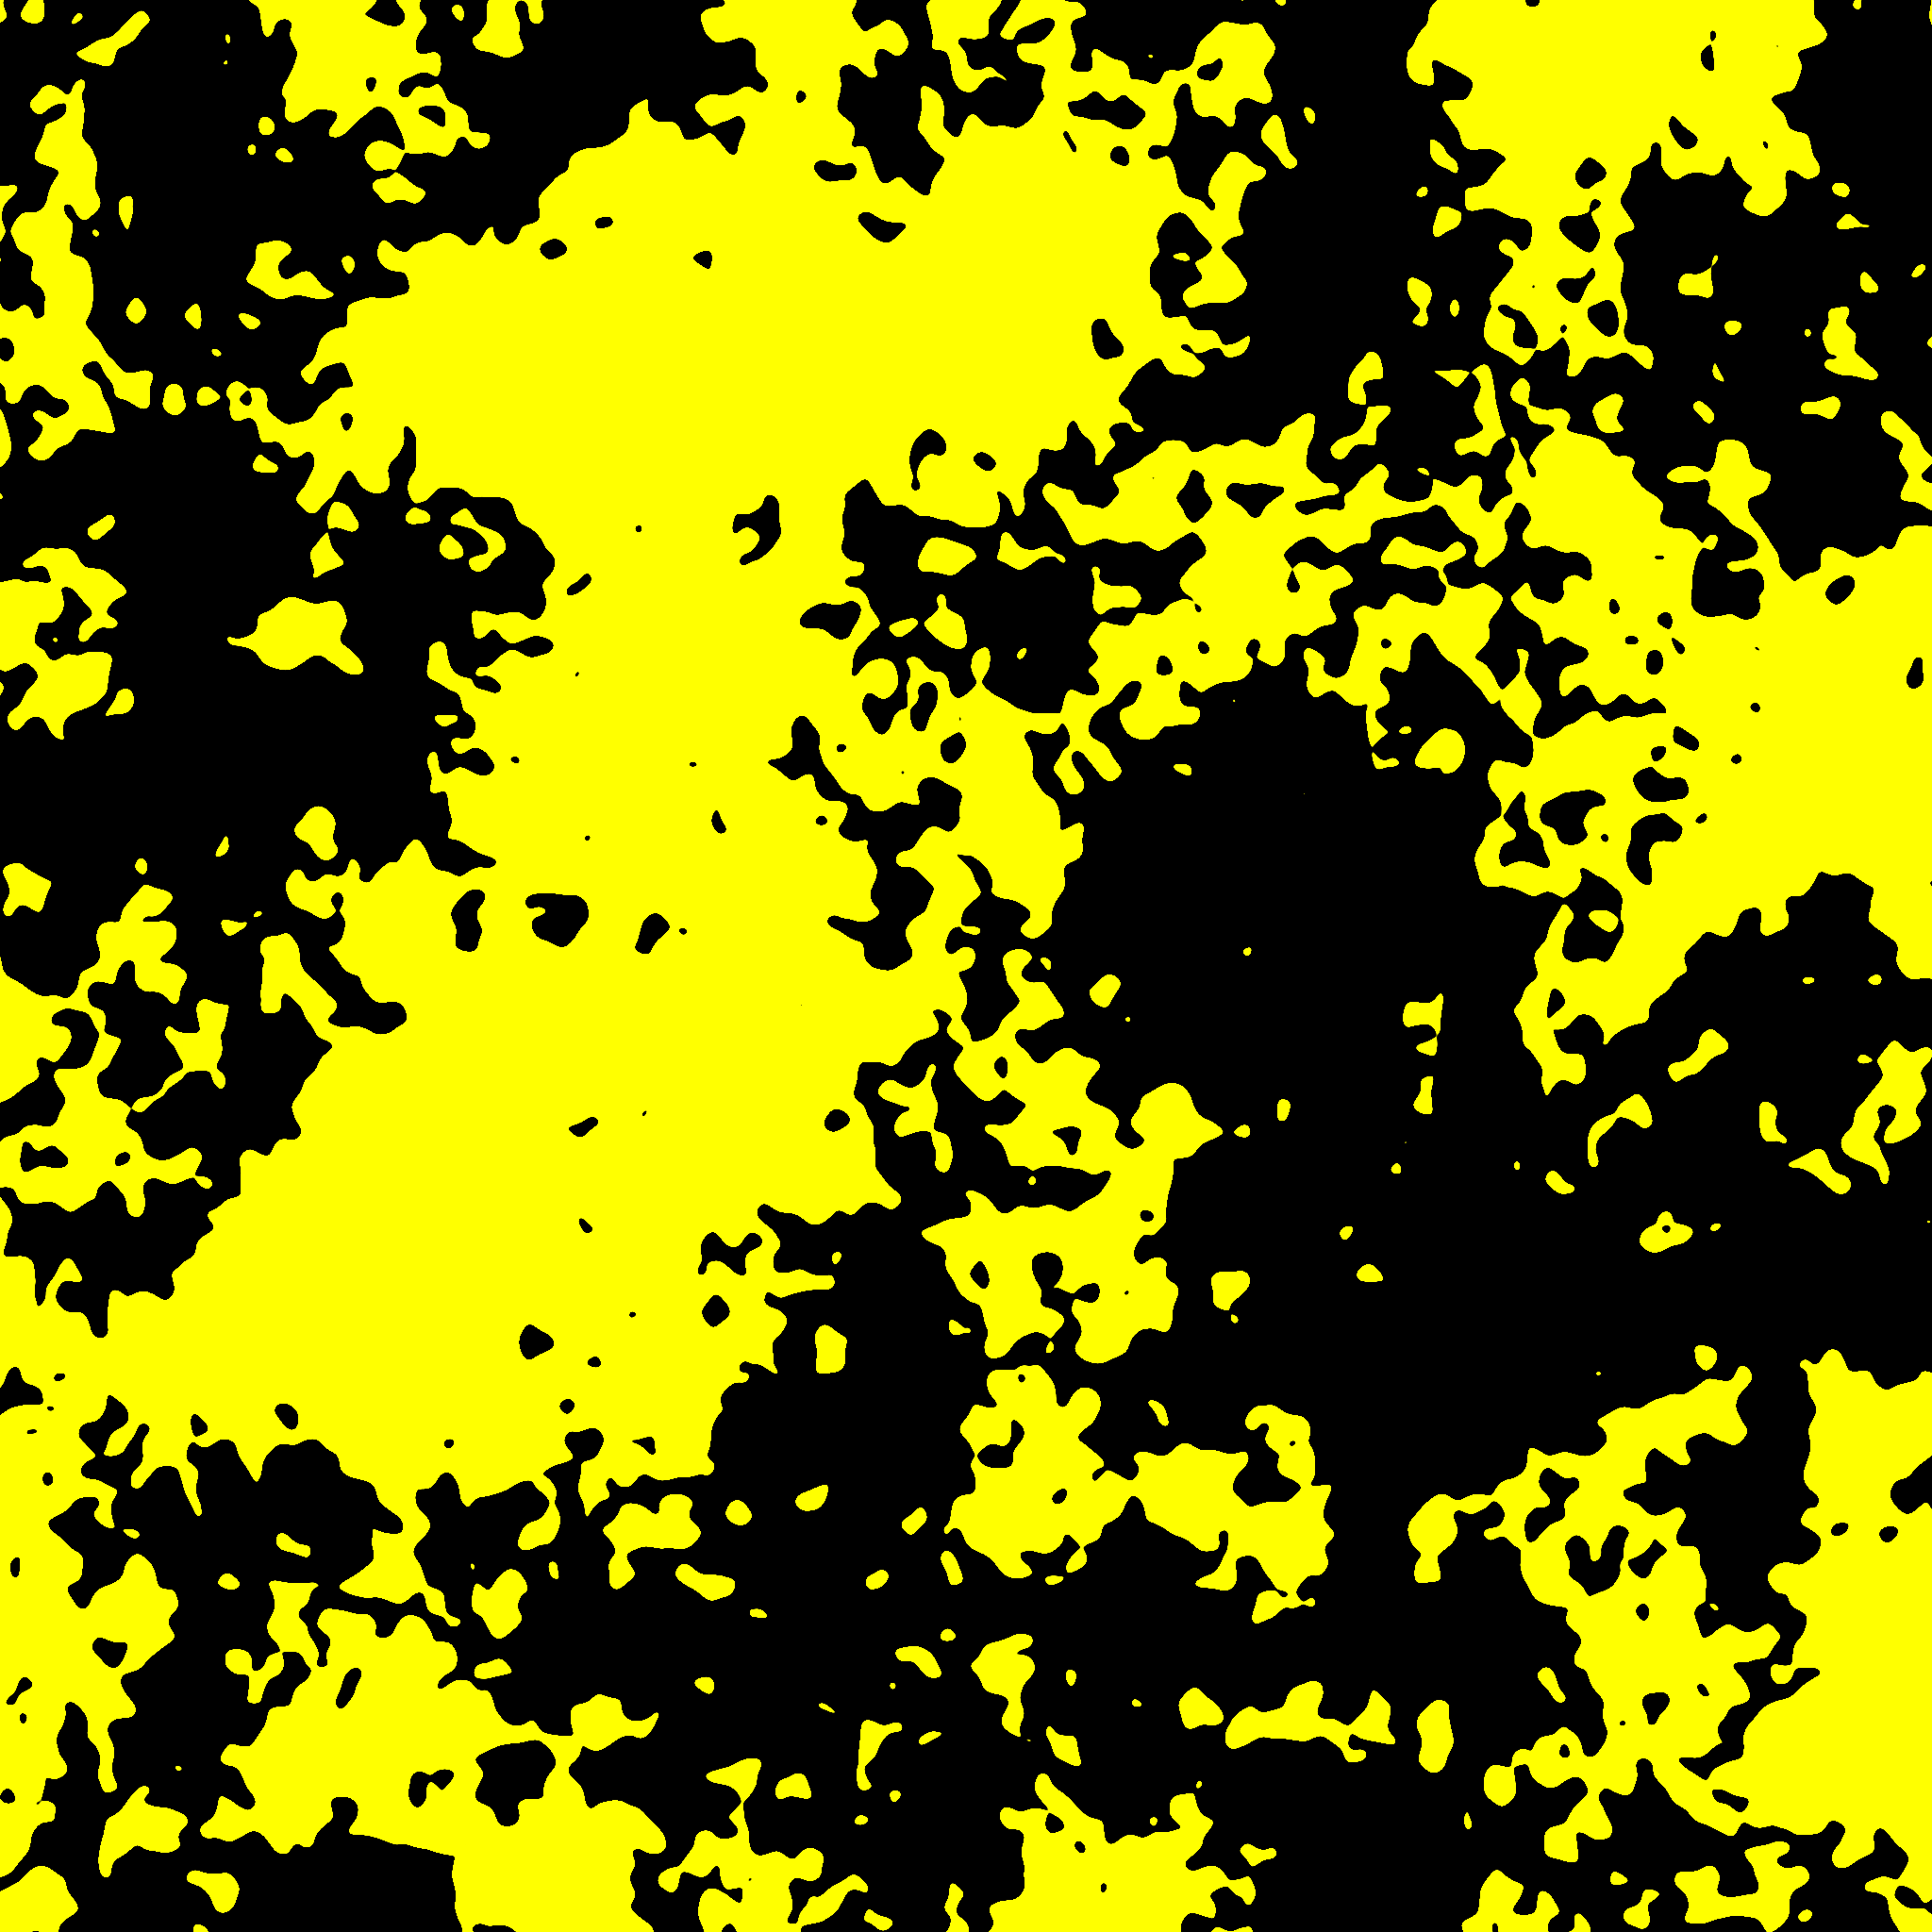
\includegraphics[width=3cm]{data/sample_perlin.png}};
      
\end{tikzpicture}}



Perlin noise najprv popíšeme matematicky a potom sa pozrieme na to, ako ho naprogramovať.
Zoberme si rovinu. Každému bodu chceme priradiť číslo tak, že čísla menšie ako $-1$ znamenajú
čiernu, čísla väčšie ako $1$ bielu a medzi nimi je spojitý prechod. Budeme tak dostávať 
obrázky ako ten nasledujúci ako vľavo. Keby sme chceli vzorku ako tá vpravo, môžeme každý bod zaokrúhliť: ak je
kladný, pixel bude žltý, ak je záporný, pixel bude čierny.\\


\centerline{
  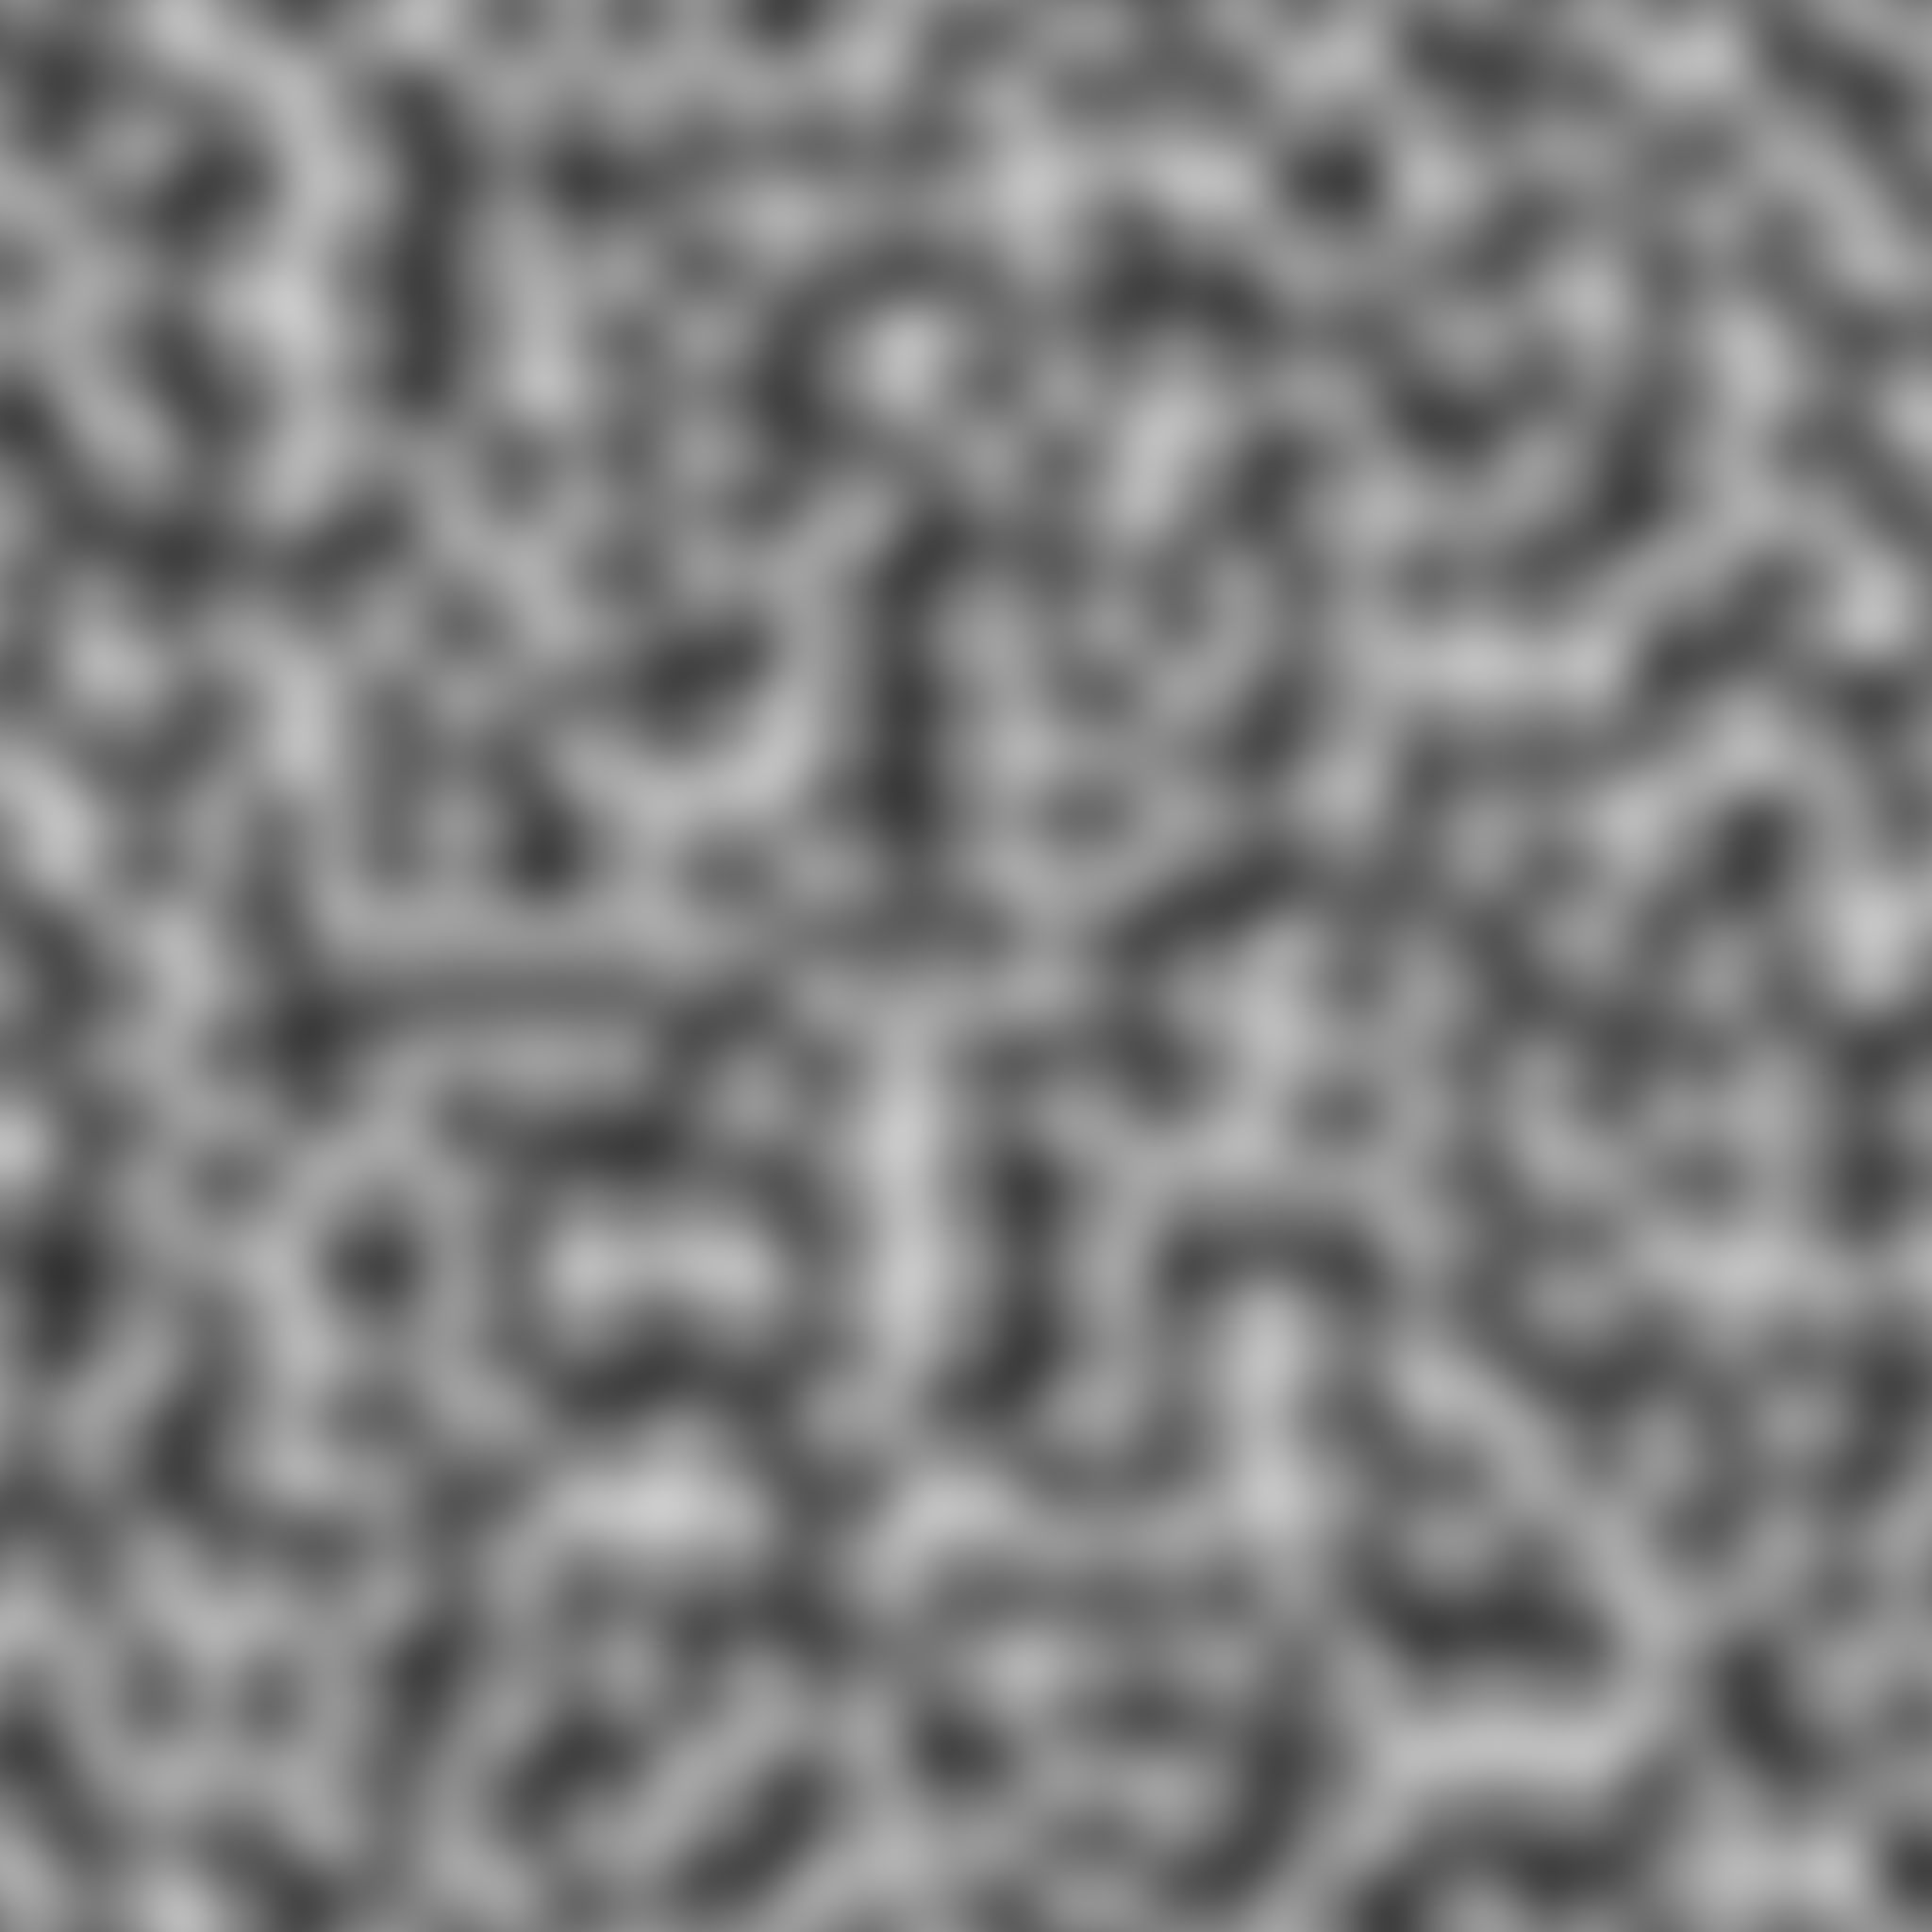
\includegraphics[width=0.4\textwidth]{data/perlin_single.png}
  \hskip 1cm
  
\includegraphics[width=0.4\textwidth]{data/perlin_single_crisp.png}
}


Základom pre vyrobenie obrázka vľavo je "natočený gradient". Zoberiem si nejaký bod $P$  a 
umiestnim doňho natočenú šípku. Tento gradient každému bodu v rovine 
priradí hodnotu podľa jeho pozície 
v smere šípky. Napr. ak mám šípku umiestnenú v bode $P=[-0.5,0.5]$, tak bodu $A$ sa
priradí číslo $0.7$ a bodu $B$ číslo $-0.4$.



\centerline{\begin{tikzpicture}[scale=1.5]
  \def\targetfill(#1)[#2]{% 
    \begin{scope}[shift={(#1)},rotate=#2]
    \shade[shading=axis,top color=white, bottom color = black, shading angle=40] 
    (0,0) circle (1);
  \end{scope}
  }
  \def\target(#1)[#2]{% 
    \begin{scope}[shift={(#1)},rotate=#2]
    \draw[red] (0,0) circle (1) (-1.5,0) -- (1.5,0);
  \draw[red,->] (0,-1.5) -- (0,1.5);
    \fill [red] (0,0) circle (0.35mm);
  \end{scope}
  }

  \def\point(#1)[#2]#3#4#5#6#7#8{
    \begin{scope}[shift={(#1)},rotate=#2]
      \coordinate (#5) at (0,#3);   
    \fill[#6] (#5) circle (0.35mm);
      \filldraw[#6, fill=#6, dashed] (#5) node[anchor=#7] {$#3$} -- ++(#4,0) 
      circle (0.35mm) node[anchor=south #8, black]{$#5$};
  \end{scope}
  }

  \coordinate (P) at (-0.5,0.5);
  \targetfill(P)[20]
  \draw[help lines, color=gray!30, dashed] (-2.9,-1.9) grid (2.9,2.9);
  \draw[->] (-3,0) -- (3,0) node[right] {$x$};
  \draw[->] (0,-2) -- (0,3) node[above] {$y$};
  \target(P)[20]
  \node[anchor=north east, red] at (P) {$P$};
  \point(P)[20]{0.7}{2.5}{A}{blue}{east}{west}
  \point(P)[20]{-0.4}{-1.5}{B}{green}{west}{east}

\end{tikzpicture}}

Výsledný obrázok získame tak, že si v rovine spravíme pravidelnú mriežku, 
v ktorej umiestnime náhodne otočené gradienty.
Každý bod roviny leží v nejakom štvorci mriežky a jeho výsledná farba sa určí kombináciou farieb zo
štyroch susedných gradientov.\\


\centerline{\begin{tikzpicture}[scale=3]
  \def\sza{0.2}
  \def\szb{0.36}
  \def\target(#1)[#2]{% 
    \begin{scope}[shift={(#1)},rotate=#2]
    \draw[red] (0,0) circle (\sza) (-\szb,0) -- (\szb,0);
  \draw[red,->] (0,-\szb) -- (0,\szb);
    \fill [red] (0,0) circle (0.15mm);
  \end{scope}
  }
  \node at (1,1) {
\includegraphics[width=6cm]{data/perlin_fixed.png}};
  \draw[help lines,color=gray!30, dashed] (0,0) grid (2,2);

  %perlin 12
  \foreach \x/\y/\a in 
  {0/0/80,0/1/140,0/2/140,1/0/280,1/1/190,1/2/30,2/0/170,2/1/90,2/2/130} {
    \target(\x,\y)[\a-90]
  }

  \coordinate (A) at (1.6,1.35);
  \filldraw[blue, dashed] (A) node[anchor=north] {$P$} circle (0.15mm) -- (1,1) (A) -- (1,2) (A) -- (2,1) (A) -- (2,2);
\end{tikzpicture}}


Kombináciu hodnôt urobíme podobne, ako sme robili interpoláciu farieb vo farebnom
gradiente v projekte o Mandelbrotovej množine,
až na to, že teraz potrebujeme interpolovať v dvoch rozmeroch (preto sa tomu hovorí {\em bilineárna interpolácia}).\indexItem{Alg}{bilineárna interpolácia}
Predstav si, že máme mriežku gradientov s krokom $d$ a chceme určiť farbu pre bod $P$ so súradnicami $[x,y]$.
Keď si všetky súradnice vydelím $d$čkom, mriežka bude mať krok $1$.
$P$ sa nachádza v mriežke medzi štyrmi bodmi $G_{00}$, $G_{10}$, $G_{01}$ a $G_{11}$.
Pripomeniem, že $\lfloor x\rfloor$ označuje celú časť z $x$, preto $G_{00}$ má súradnice
$\left\lfloor\frac{x}{d}\right\rfloor,\left\lfloor\frac{y}{d}\right\rfloor$ a ostatné 
4 body sú vždy o $1$ ďalej.


\centerline{\begin{tikzpicture}[scale=5.5]
  \def\ofs{0.2}
  \def\ofsi{0.35}
  \def\lclr{teal}
  \tikzstyle{link}=[dashed, thin, \lclr, shorten <= -0.6ex]
  \def\dot(#1)[#2]{\fill[#2] (#1) circle (0.007);}
  % pozicia, uhol, dlzka od-do, vyska, nazov suradnice
  \def\grr(#1)[#2](#3,#4)#5{
    \begin{scope}[shift={(#1)},rotate=#2]
      \draw[red] (-0.1,0) -- (0.1,0) (0,0) circle (0.05);
      \draw[->,red] (0,#3) -- (0,#4);
      \coordinate (#5) at ($(0,-100)!(P)!(0,100)$);
    \end{scope}
  }
  \draw[dashed] (0,0-\ofsi) node [below] {$\left\lfloor\frac{x}{d}\right\rfloor$} -- (0,0);
  \draw[dashed] (1,0-\ofsi) node [below] {$\left\lfloor\frac{x}{d}\right\rfloor+1$} -- (1,0);
  \draw[dashed] (1+\ofsi,0) node [right] {$\left\lfloor\frac{y}{d}\right\rfloor$} -- (1,0);
  \draw[dashed] (1+\ofsi,1) node [right] {$\left\lfloor\frac{y}{d}\right\rfloor+1$} -- (1,1);

  \draw (0-\ofs,0) -- (1+\ofs,0) (0-\ofs,1) -- (1+\ofs,1) (0,0-\ofs) -- (0,1+\ofs) (1,0-\ofs) -- (1,1+\ofs);
  \node[anchor = north east, inner sep=0.5cm] at (0,0) {$G_{00}$} ;
  \node[anchor = north west, inner sep=0.5cm] at (1,0) {$G_{10}$} ;
  \node[anchor = south east, inner sep=0.5cm] at (0,1) {$G_{01}$} ;
  \node[anchor = south west, inner sep=0.5cm] at (1,1) {$G_{11}$} ;
  

  \coordinate (P) at (0.43,0.6);
  
  \grr(0,0)[19](-0.15,0.5){v00} 
  \draw[link] (v00) node[anchor=north west] {$v_{00}$} -- (P);
  \dot(v00)[\lclr]
  
  \grr(1,0)[-30](-0.15,0.3){v10}
  \draw[link] (v10) node[anchor=north west] {$v_{10}$} -- (P);
  \dot(v10)[\lclr]

  \grr(0,1)[-62](-0.15,0.3){v01}
  \draw[link] (v01) node[anchor=south east] {$v_{01}$} -- (P);
  \dot(v01)[\lclr]

  \grr(1,1)[-130](-0.3,0.2){v11}
  \draw[link] (v11) node[anchor=south west] {$v_{11}$} -- (P);
  \dot(v11)[\lclr]


  \draw[blue,brace=1mm/](0,1.2)-- node[above=2.5ex]{$1$}(1,1.2);

  \coordinate (Px) at ($($(0,0)!(P)!(1,0)$) + (0,0-\ofs)$);
  \coordinate (Py) at ($($(0,0)!(P)!(0,1)$) + (0-\ofs,0)$);
 
  \draw[thin,lightgray]  (Px) -- ($(0,1)!(P)!(1,1)$)  (P)--(Py);
  \draw[blue,brace=1mm/mirror] (0,0-\ofs) -- node[below=2.5ex]{$r=\frac{x}{d}-\left\lfloor\frac{x}{d}\right\rfloor$} (Px);
   \draw[blue,brace=1mm/mirror] (Px) -- node[below=2.5ex]{$1-r$} (1,0-\ofs);

   \draw[blue,brace=1mm/] (0-\ofs,0) -- node[left=2.5ex]{$s=\frac{y}{d}-\left\lfloor\frac{y}{d}\right\rfloor$} (Py);
   \draw[blue,brace=1mm/] (Py) -- node[left=2.5ex]{$1-s$} (0-\ofs,1);

  \dot(P)[black]
  \node[anchor=west] at (P){$P\;\left[\frac{x}{d},\frac{y}{d}\right]$};
  \fill ($(0,0)!(P)!(1,0)$) node[anchor = north west]{$C$} circle (0.007)
   ($(0,1)!(P)!(1,1)$) node[anchor = south west]{$D$} circle (0.007);
\end{tikzpicture}}
%\pagebreak[1]


Predpokladajme, že sme už vyrátali hodnoty, ktoré prislúchajú bodu $P$ v
jednotlivých gradientoch a označili sme si ich
$v_{00}$, $v_{10}$, $v_{01}$ a $v_{11}$. Ako z nich skombinovať výslednú hodnotu v $P$? 
Desatinná časť po vydelení $x/d$ 
je $r=\frac{x}{d}-\left\lfloor\frac{x}{d}\right\rfloor$. Keby si bod $P$
posúval v štvorci zľava doprava, hodnota $r$ sa bude plynule meniť medzi $0$ a $1$.
Preto hodnotu v bode $C$ vieme interpolovať ako $v_C=v_{00}(1-r)+v_{10}r$. 
Podobne hodnotu v bode $D$ interpolujeme
$v_D=v_{01}(1-r)+v_{11}r$. 
Napokon urobíme rovnakým spôsobom interpoláciu medzi $v_C$ a $v_D$ v smere osi $y$, 
takže výsledok bude $v_C(1-s)+v_Ds$. 


Skoro dobré, ale  je tam stále drobný
problém: pretože interpolujeme lineárne iba v rámci jedného štvorca,
vznikajú nám nepekné zlomy ako vľavo, kým my potrebujeme hladký prechod ako vpravo\\


\centerline{
  
\includegraphics[width=0.4\textwidth]{data/perlinL_fixed.png}
  \hskip 1cm
  
\includegraphics[width=0.4\textwidth]{data/perlin_fixed.png}
}

\phantom{a}
\hfill
\begin{tikzpicture}
\begin{axis}[
  width=60mm, 
  height=6cm,
  domain=0:1,
  xmin=0,
  xmax=1,
  ymin=0,
  ymax=1,
  xlabel=$r$,
  /pgf/number format/.cd,
        1000 sep={}
]
  \addplot[no markers,red!50!white]{x};
  \addplot[no markers,green!50!white]{1-x};
\end{axis}
\end{tikzpicture}
  \hfill
\begin{tikzpicture}
\begin{axis}[
  width=60mm, 
  height=6cm,
  domain=0:1,
  xmin=0,
  xmax=1,
  ymin=0,
  ymax=1,
  xlabel=$6r^5-15r^4+10r^3$,
  /pgf/number format/.cd,
        1000 sep={}
]
  \addplot[no markers,red!50!white]{x * x * x * (10 + x * (6 * x - 15))};
  \addplot[no markers,green!50!white]{1-x * x * x * (10 + x * (6 * x - 15))};
\end{axis}
\end{tikzpicture}
\hfill
\phantom{a}


Hladký prechod sa dá dosiahnuť tak, že namiesto interpolácie s parametrami $r$ a $1-r$, ktoré
sú pri koncoch špicaté, budeme interpolovať s parametrami $f(r)$ a $1-f(r)$ pre nejakú
vhodnú funkciu $f$, ktorá je na koncoch hladká. Perlin odporúča zobrať 
$f(r)=6r^5-15r^4+10r^3$. Môžeme aj tak, prečo nie.

 
Teraz môžeme napísať takmer celý program na Perlin noise. 
Najprv si urobím pomocnú funkciu na lineárnu interpoláciu \vb{lerp}, ktorá sa
bude hodiť vo všeobecnejšej podobe


\begin{lstlisting}
template <typename T>
T lerp(const T& v0, const T& v1, double t) {
  return (1 - t) * v0 + t * v1;
}
\end{lstlisting}


Teraz vyrobím triedu \vb{Perlin},
ktorá bude mať dva parametre: \vb{n} veľkosť obrázka (pre jednoduchosť budem
robiť štvorcové obrázky rozmerov $n\times n$) a krok mriežky \vb{d}.
Zavolanie konštruktora vyrobí tabuľku \vb{H}, v ktorej bude výsledná výšková
mapa. Na natočené šípky budem mať triedu \vb{Vec} o ktorej si povieme viac o 
chvíľu, nateraz si ju predstav ako 


\begin{lstlisting}
struct Vec {
  double x, y;
};
\end{lstlisting}


Natočené šípky budú uložené v tabuľke $G$ rozmerov $m\times m$, kde 
$m=1+\left\lfloor\frac{n}{d}\right\rfloor$. V konštruktore
najprv vygenerujeme náhodné šípky tak, že zvolíme náhodný uhol \vb{theta} ($\theta$)
a šípka bude ukazovať do bodu so súradnicami $[\cos(\theta),\sin(\theta)]$
(o funkciách $\sin$ a $\cos$ pozri odbočku v kapitole~\ref{sect:editor}).
Potom už len vyrátam pre každý bod $P=[i,j]$ jeho farbu.
To znamená, že keď vyrobím premennú typu \vb{Perlin}, konštruktor vyrobí tabuľku \vb{H},
ku ktorej potom môžem pristupovať.


\begin{lstlisting}
struct Perlin {
  int n, d, m;  
  Tabulka<double> H;
  Tabulka<Vec> G;

  // konštruktor. 
  // všimni si zápis n\{\_n\} - niekedy je čitateľnejšie volať copy konštruktor 
  // pre int za dvojbodkou ako písať priradenie v tele konštruktora
  Perlin(int _n, int _d) : n{_n}, d{_d}, m{1 + n / d}, 
                           H(n, n), G(m, m) {
    for (int i = 0; i < m; i++)
      for (int j = 0; j < m; j++) {
        double theta = dis(rnd) * M_PI * 2.0;
        G(i, j) = {cos(theta), sin(theta)};
      }

    for (int i = 0; i < n; i++)
      for (int j = 0; j < n; j++) {
        // bod P so súradnicami [i,j]
        Vec p{ (double)i / (double)d,  (double)j / (double)d};

        // súradnice bodu G00
        int o[2] = {(int)p.x, (int)p.y}; 

        // hodnoty v00, v10, v01 a v11
        double v[4];

        ... // tu ich treba nejak vyrátať
        
        double r = fade(p.x - o[0]), s = fade(p.y - o[1]);
        double vc = lerp(v[0], v[1], r), vd = lerp(v[2], v[3], r);
        H(i, j) = lerp(vc, vd, s);
      }
  }

  // fade funkcia, ako ju odporúčal Perlin
  double fade(double t) {
    return t * t * t * (10 + t * (6 * t - 15));
  }
};
\end{lstlisting}


Ostáva doplniť posledná vec, a to ako vyrátať hodnoty $v_{00},\ldots,v_{11}$,
teda ako pre daný bod zrátať jeho výšku v nejakom natočenom gradiente. 
Predtým sa ale hodí

\section*{Matematické intermezzo: o bodoch a vektoroch}
\label{mat.body}

\indexItem{Mat}{bod, vektor}
Bod v rovine je vec, ktorá má dve súradnice, $x$ a $y$. Ak mám dva body, napr.
$A[x,y]$, $B[x',y']$, tak najkratšia cesta z bodu $A$ do bodu $B$ je úsečka, ktorá
sa v smere osi $x$ pohne o $x'-x$ a v smere osi $y$ o $y'-y$. Takýto úsečka
sa volá prenášač\indexItem{Mat}{vektor ako rozdiel bodov, sčitovanie vektorov} 
({\em vektor}) a dá sa zapísať dvoma číslami pre posun v $x$-ovom
a $y$-ovom smere, takže vyzerá
rovnako ako bod so súradnicami $[x'-x,y'-y]$. Je preto prirodzené
si to predstaviť tak, že ak odčítam od seba dva body, dostanem vektor.
Ak treba body a vektory rozlíšiť, nad vektory sa niekedy
zvykne písať šípka, napr. vektor $v$ je $\vec v = B-A$. 
Podobne keď k nejakému bodu $C$ prirátame vektor $\vec v$, 
dostaneme nový bod (ten, do ktorého nás
vektor prenesie).


\centerline{
\begin{tikzpicture}[scale=0.5]
  \tikzstyle{vecs}= [-{>[length=2ex,width=1.7ex]}]
  \def\dot(#1){\fill (#1)circle (1.8pt) }
  \draw[dotted,thin,gray] (-1,-1) grid (12,8);
  \coordinate (A) at (1,3);
  \coordinate (B) at (8,6);
  \draw[red,style=vecs](A) -- node[anchor = south east, inner sep=2mm]{$\vec v=B-A$}(B);
  \dot(A) node[anchor=north east]{$A$};
  \dot(B) node[anchor=south west]{$B$};
  \draw[thin, teal, dashed] 
  (A) -- ++(3,-2) coordinate (AA)
  (B) -- ++(3,-2) coordinate (BB);
  \draw[magenta, style = vecs] (AA) -- (BB);
  \dot(AA) node[anchor=north]{$C$};
  \dot(BB) node[anchor=north west]{$C+\vec v$};
  \draw[thin] (-1.5,0) -- (12.5,0) (0,-1.5) -- (0,8.5);
\end{tikzpicture}}

Vektory môžeme sčitovať prirodzeným spôsobom po zložkách (t.j. 
$[x,y]+[x',y']=[x+x',y+y']$), čo sa dá nakresliť ako skladanie šípok: na konci jednej
nakreslíme druhú:


\centerline{
\begin{tikzpicture}[scale=0.5]
  \tikzstyle{vecs}= [-{>[length=2ex,width=1.7ex]}]
  \def\dot(#1){\fill (#1)circle (1.8pt) }
  \draw[dotted,thin,gray] (-1,-1) grid (12,8);
  \coordinate (A) at (1,1);
  \coordinate (B) at ($(A)+(6,2)$);
  \coordinate (C) at ($(B)+(3,5)$);
  \dot(A); \dot(B); \dot(C);
  \draw[orange,style=vecs](A) -- node[anchor = north west, inner sep=1mm]{$\vec u=[6,2]$}(B);
  \draw[teal,style=vecs](B) -- node[anchor = north west, inner sep=1mm]
  {$\vec v=[3,5]$}(C);
  \draw[magenta,style=vecs](A) -- node[anchor = south east, inner sep=1mm]
  {$\vec u+\vec v=[9,7]$}(C);
  \draw[thin] (-1.5,0) -- (12.5,0) (0,-1.5) -- (0,8.5);
\end{tikzpicture}}


Rovnako dobre dáva zmysel, aby sme vektor vynásobili číslom: napr. ak 
$\vec v=[x,y]$, tak $4.2\cdot\vec v=[4.2x,4.2y]$ je
šípka v rovnakom smere ako $\vec v$, iba $4.2$-krát dlhšia. Podobne $-0.5\cdot\vec v$ je
šípka polovičnej dĺžky a v opačnom smere. 


Ak mám bod $A[x,y]$, tak si viem povedať, že to je vlastne vektor $A-[0,0]$, t.j.
šípka, ktorá ukazuje zo začiatku súradnicovej sústavy do $A$. Teraz je bod a vektor naozaj
to isté. Premysli si to: napr. $[9,7]-[3,5]=[6,2]$ môžem interpretovať tak, že mám bod
so súradnicami $[9,7]$ a bod so súradnicami $[3,5]$, tak vektor medzi nimi má súradnice $[6,2]$.
Ale rovnako môžem povedať, že ak mám vektor $[3,5]$, tak $-[3,5]$ je rovnako dlhý vektor v 
opačnom smere a $[9,7]+(-[3,5])$ je skladanie vektorov, ktorého výsledkom je vektor $[6,2]$.


Z Pytagorovej vety viem, že ak $\vec v$ je vektor so súradnicami $[x,y]$, tak jeho 
dĺžka je $\nrm{\vec v}=\sqrt{x^2+y^2}$. Ak obe súradnice vydelím dĺžkou, dostanem vektor
$\vec v'=\left[\frac{x}{\nrm{\vec v}},\frac{y}{\nrm{\vec v}}\right]$, ktorého dĺžka je 
$$\nrm{\vec v'}=\sqrt{\left(\frac{x}{\nrm{\vec v}}\right)^2+\left(\frac{y}{\nrm{\vec v}}\right)^2}
=\sqrt{\frac{x^2}{\nrm{\vec v}^2}+\frac{y^2}{\nrm{\vec v}^2}}
=\sqrt{\frac{1}{\nrm{\vec v}^2}(x^2+y^2)}=\sqrt{\frac{1}{\nrm{\vec v}^2}}\sqrt{x^2+y^2}=
\frac{1}{\nrm{\vec v}}\nrm{\vec v}=1
$$
Hovoríme, že $\vec v'$ je {\em normovaný} (resp. {\em normalizovaný}) vektor.\indexItem{Mat}{normalizovaný vektor}


\centerline{
\begin{tikzpicture}[scale=0.5]
  \tikzstyle{vecs}= [-{>[length=2ex,width=1.7ex]}]
  \def\dot(#1){\fill (#1)circle (1.8pt) }
  \draw[dotted,thin,gray] (-1,-1) grid (12,8);
  \coordinate (A) at (9,7);
  \draw[magenta, style=vecs] (0,0) -- (A) node[anchor=south west]{$\vec v = [x,y]$};
  \dot(0,0); \dot(A);
  \draw[thin] (-1.5,0) -- (12.5,0) (0,-1.5) -- (0,8.5);
  \draw[thin,gray](A) -- ($(0,0)!(A)!(10,0)$) coordinate(Ax);
  \draw[brace=1mm/] (A) -- node[anchor=west, xshift=2ex]{$y$} (Ax);
  \draw[thick, teal, style=vecs] (0,0) -- node[anchor=south east]{$1$}
  ($0.4*(A)$) coordinate(B) node[anchor=south east]{$\vec v'$};
  \dot(B);
  \draw[thin,gray](B) -- ($(0,0)!(B)!(10,0)$) coordinate(Bx);
  \draw[brace=1mm/] (B) -- node[anchor=west, xshift=2ex]{$\frac{y}{\nrm{\vec v}}$} (Bx);
\end{tikzpicture}}


Máme teda vektory, ktoré vieme sčitovať, odčitovať a násobiť reálnym číslom. Samozrejme, toto
všetko by rovnako dobre fungovalo v troch (a viacerých) rozmeroch. Môžeme ale nejak rozumne
vynásobiť dva vektory medzi sebou? 
Tu to už nie je také jednoznačné. Môžme vymyslieť rôzne 
operácie, ktoré nazveme súčin, a ktoré budú mať rôzne vlastnosti podľa toho, čo práve potrebujeme počítať. 
Jeden spôsob je uvedomiť si, že vektor v rovine so súradnicami $[x,y]$
je vlastne komplexné číslo $x+iy$, takže môžeme používať násobenie ako pri komplexných číslach.
Ukážem ti ešte dva iné spôsoby, ktoré sa nám budú hodiť, a to tzv.  {\em skalárny} a {\em vektorový} súčin.


\indexItem{Mat}{skalárny súčin}
Skalárny súčin je spôsob násobenia, ktorý je veľmi prirodzený napr. vo fyzike. Možno vieš, že fyzikálna
veličina {\em práca} je súčin sily a dráhy, t.j. ak pôsobí na teleso sila $1$N a posunie ho tým o $1$m,
vykoná pri tom prácu $1$J. Zvyčajne sa to zapisuje $W=Fd$.


\centerline{
  \begin{tikzpicture}[scale=1] 
  \draw[white] (0,0) -- (0,-0.8);
    \definecolor{acol}{rgb}{0.85,0.85,0.95}
    \node[xscale=-1,yscale=1,inner sep=0pt, anchor = south] (auto) at (2.7,0) {\textcolor{acol}{\usymH{1F69A}{1cm}}};    
    \node[xscale=-1,yscale=1,cyan!50!white,anchor=south, inner sep=0pt] (vlak) at (0,0) {\usymH{1F683}{1cm}};
    \draw[draw=acol, shorten <= 0.68cm, shorten >= 0.5cm, line width=0.6mm] 
    ($(vlak.center)+(0,-0.2)$) -- ($(auto.center)+(0,-0.2)$);
  %\node[xscale=-1,yscale=1,blue,anchor=south, inner sep=0pt] at (5,3) {\usymH{1F681}{1cm}};

    \draw (-1.5,0) -- (6,0);
  \foreach \x in {0,...,5}
  \draw (\x,-0.1) -- (\x,0.1);
    \fill[red] (vlak.center) circle (0.8mm);
    \draw[red,line width=0.6mm,->,>=latex] (vlak.center) -- node[above]{$F$} ++(3,0);
    \draw[cyan,line width = 0.6mm,->,>=latex] (0,-0.4) -- node[below]{$d$} (5,-0.4);
    \fill[cyan] (0,-0.4) circle (0.8mm);

\end{tikzpicture}
}


Tu sa ale potichu predpokladá, že sila aj dráha sú čísla, a preto ich môžem násobiť. Lenže v skutočnosti sila aj dráha sú
vektory a môžu pôsobiť rôznym smerom


\centerline{
  \begin{tikzpicture}[scale=1] 
  \draw[white] (0,0) -- (0,-0.8);
    \definecolor{acol}{rgb}{0.85,0.85,0.95}
   % \node[xscale=-1,yscale=1,inner sep=0pt, anchor = south] (auto) at (2.7,0) {\textcolor{acol}{\usymH{1F69A}{1cm}}};    
    \node[xscale=-1,yscale=1,blue,anchor=south, inner sep=0pt] (heli) at (4,2.5) {\textcolor{acol}{\usymH{1F681}{1cm}}};
    \node[xscale=-1,yscale=1,cyan!50!white,anchor=south, inner sep=0pt] (vlak) at (0,0) {\usymH{1F683}{1cm}};
    \draw[draw=acol, shorten <= 0.8cm, shorten >= 0.3cm, line width=0.6mm] 
    (vlak.center) -- ($(heli.center)+(0,-0.3)$) coordinate (lano);

    \draw (-1.5,0) -- (6,0);
  \foreach \x in {0,...,5}
  \draw (\x,-0.1) -- (\x,0.1);
    \draw[cyan,line width = 0.6mm,->,>=latex] (vlak.center) -- node[below]{$\vec d$} ++(5,0) coordinate (endD);
    \draw[red,line width=0.6mm,->,>=latex] (vlak.center) -- node[above]{$\vec F$} ($(vlak.center)!0.8!(lano)$) 
    coordinate(endF);
    \draw[thin, gray, dashed] (endF) -- ($(vlak.center)!(endF)!(endD)$) coordinate(fin);
    \draw[thin, ->, >=latex ] (vlak.center) -- (fin);
    \def\len{0.95cm}
    \draw[thin] ($(vlak.center)!\len!(endD)$) arc(0:28:\len);
    \fill[red] (vlak.center) circle (0.8mm);
\end{tikzpicture}
}


V tomto prípade sa časť sily, ktorou pôsobí vrtuľník, vyplytvá na nadľahčovanie vagóna a prácu robí 
iba tá časť, ktorá je rovnobežná s dráhou, takže na vyrátanie práce násobím
dĺžku vektora $\vec d$ a priemetu $\vec F$ (čierna šípka na obrázku). 
Aby sa zachoval rovnaký zápis, chcel by som násobiť vektory tak,
aby som mohol napísať $W=\vec F\cdot\vec d$. Ako sa také násobenie dá urobiť? Výsledkom násobenia dvoch vektorov
musí byť číslo, ktoré vznikne vynásobením dĺžky jedného a priemetu druhého:


\centerline{
\begin{tikzpicture}[scale=0.5]
  \tikzstyle{vecs}= [-{>[length=2ex,width=1.7ex]}]
  \def\dot(#1){\fill (#1)circle (1.8pt) }
  \draw[dotted,thin,gray] (-1,-1) grid (12,7);
  %\draw[thin] (-1.5,0) -- (12.5,0) (0,-1.5) -- (0,8.5);
  \def\degi{20}
  \def\degii{40}
  \coordinate (A) at (\degi:12cm);
  \coordinate (B) at ($(0,0)!7.5cm!\degii:(A)$);
  \draw[magenta, vecs] (0,0) -- node[pos=0.8, below]{$\vec u$}(A);
  \draw[teal, vecs] (0,0) -- node[anchor = east]{$\vec v$}(B);
  \coordinate (Bx) at ($ (0,0)!(B)!(A) $);
  \draw[thin,gray] (B) -- (Bx)
     ($(0,0)!1.5cm!(A)$) arc (\degi:\degi+\degii:1.5cm)
     ($(Bx)!4mm!(0,0)$) arc (180+\degi:90+\degi:4mm)
     ;
  \node at ($(0,0)!1cm!0.5*\degii:(A)$) {$\alpha$};
  \draw[teal, brace=1mm/mirror](0,0) -- node[rotate=\degi,below=2mm]{$\nrm{\vec v}\cos(\alpha)$} (Bx);
  \dot(0,0);\dot(A);\dot(B);
\end{tikzpicture}}


Výsledok by teda mal byť $\vec u\cdot\vec v=\nrm{\vec u}\cdot\nrm{\vec v}\cdot\cos(\alpha)$, kde $\alpha$ označuje
uhol, ktorý tie dva vektory zvierajú. Teraz idem trochu počítať a na záver mi vyjde, že takýto skalárny
súčin sa dá veľmi jednoducho vyrátať. Tak poďme na to. Zoberme si vektory $\vec u$, $\vec v$ ako na predchádzajúcom obrázku
a označme si $a=\nrm{\vec u}$, $b=\nrm{\vec v}$, $p=b\cos(\alpha)$. Situácia teda vyzerá takto:


\centerline{
\begin{tikzpicture}[scale=0.5]
  \tikzstyle{vecs}= [-{>[length=2ex,width=1.7ex]}]
  \def\dot(#1){\fill (#1)circle (1.8pt) }
  \draw[dotted,thin,gray] (-1,-1) grid (12,7);
  %\draw[thin] (-1.5,0) -- (12.5,0) (0,-1.5) -- (0,8.5);
  \def\degi{20}
  \def\degii{48}
  \coordinate (A) at (\degi:12cm);
  \coordinate (B) at ($(0,0)!6cm!\degii:(A)$);
  \draw[magenta] (0,0) -- node[pos=0.8, below]{$a$}(A);
  \draw[teal] (0,0) -- node[anchor = east]{$b$}(B);
  \coordinate (Bx) at ($ (0,0)!(B)!(A) $);
  \draw[thin,gray] (B) -- node[anchor=west] {$c$} (Bx)
     ($(0,0)!1.5cm!(A)$) arc (\degi:\degi+\degii:1.5cm)
     ($(Bx)!4mm!(0,0)$) arc (180+\degi:90+\degi:4mm)
     (B) -- node [anchor=south west]{$d$} (A)
     ;
  \node at ($(0,0)!1cm!0.5*\degii:(A)$) {$\alpha$};
  \draw[teal, brace=1mm/mirror](0,0) -- node[rotate=\degi,below=2ex]{$p$} (Bx);
  \dot(0,0);\dot(A);\dot(B);
  \node[anchor=north east] at (0,0) {$[0,0]$};
  \node[anchor=west] at (A) {$[u_x,u_y]$};
  \node[anchor=south] at (B) {$[v_x,v_y]$};
\end{tikzpicture}}


\tikzexternaldisable
\def\mathnode(#1)#2{\tikz[remember picture,baseline=(#1.base)]\node[draw=none, inner sep=0pt, outer sep=0pt](#1){$#2$};}

Potrebujeme vyrátať skalárny súčin $\nrm{\vec u}\cdot\nrm{\vec v}\cdot\cos(\alpha)$, t.j. v našom označení
$ap$. Všimneme si dva pravouhlé trojuholníky: jeden so stranami $b$, $p$, $c$ a druhý so stranami $d$, $a-p$, $c$.
Z Pytagorovej vety dostaneme pre prvý z nich $p^2=b^2-c^2$ a pre druhý $c^2=d^2-(a-p)^2$. Keď to dáme dokopy,
dostaneme $p^2=b^2-d^2+(a-p)^2$. Teraz roznásobíme $(a-p)^2=(a-p)\cdot(a-p)=a^2-2ap+p^2$, takže máme
$$p^2=b^2-d^2+a^2-2ap+p^2$$
a teda
$$2ap=\mathnode(b){b^2}+\mathnode(a){a^2}\mathnode(d){-d^2}$$
Teraz si dosadím $b^2=\nrm{\vec v}^2=v_x^2+v_y^2$, $a^2=\nrm{\vec u}^2=u_x^2+u_y^2$  a 
$d^2=(u_x-v_x)^2+(u_y-v_y)^2$ a dostanem
$$2ap=\mathnode(bb){v_x^2+v_y^2}+\mathnode(aa){u_x^2+u_y^2}\mathnode(dd){-(u_x-v_x)^2-(u_y-v_y)^2}$$

\begin{tikzpicture}[remember picture, overlay, draw opacity=0.6] 
  \def\spoj[#1]#2#3{
  \node[fit=(#2),draw=#1, rounded rectangle,inner xsep=0] (tmp1) {};
  \node[fit=(#3),draw=#1, rounded rectangle,inner xsep=0] (tmp2) {};
  \draw[#1] (tmp1)--(tmp2);
 }
  \spoj[teal]b{bb}
  \spoj[magenta]a{aa}
  \spoj[blue]d{dd}
\end{tikzpicture}
\tikzexternalenable



Keď si roznásobím $(u_x-v_x)^2=u_x^2-2u_xv_x+v_x^2$ a $(u_y-v_y)^2=u_y^2-2u_yv_y+v_y^2$ a dosadím,
dostanem
$$ap=u_xu_y+v_xv_y$$


Takže si to zhrňme: ak mám dva vektory $\vec u=[u_x,u_y]$ a $\vec v=[v_x,v_y]$, tak\\
\phantomsection\label{page:dotproduct-angle}

\centerline{\fbox{
  $\vec u\cdot\vec v=\nrm{\vec u}\cdot\nrm{\vec v}\cdot\cos(\alpha) = u_xu_y + v_xv_y$}}


Toto sa často hodí, lebo $u_xu_y + v_xv_y$ sa dá zrátať ľahko a rýchlo a ak sú $\vec u$ a $\vec v$ normované,
čiže ich dĺžka je $1$, tak priamo vyrátam kosínus uhla medzi nimi. 
Keď si nakreslím, ako závisí kosínus od veľkosti uhla, dostanem známy obrázok


\centerline{
\begin{tikzpicture}
\begin{axis}[
  width=0.6*\textwidth, 
  height=5cm,
  axis x line=middle,
  axis y line=left,
  axis line style={-},
  xtick={0,90,...,360},  
  xlabel=$\alpha$,
  xticklabel={\pgfmathtruncatemacro{\tmp}{\tick}$\tmp^\circ$},
  ylabel=$\cos(\alpha)$,
  scaled x ticks=false,
  scaled y ticks=false,
  domain=0:360,
  xmin=0,
  xmax=360,
  ymin=-1.1,
  ymax=1.1,
  /pgf/number format/.cd,
        1000 sep={}
]
  \addplot[dashed,very thin,gray!50!white]{1};
  \addplot[dashed,very thin,gray!50!white]{-1};
  \addplot[samples=1000,no markers,red!50!white]{cos(x)};
\end{axis}
\end{tikzpicture}}


Špeciálne, viem rýchlo zistiť, či sú dva vektory
kolmé: stačí overiť, či ich skalárny súčin je rovný nule. A, samozrejme, síce sme to všetko rátali v rovine, 
ale pre trojrozmerné vektory by to fungovalo úplne rovnako.


\indexItem{Mat}{vektorový súčin}
Iný spôsob súčinu, ktorý sa ale dá použiť iba pre trojrozmerné vektory, je tzv. {\em vektorový súčin}. 
Ak máš rovinu v 3D priestore  (napr. list papiera na stole) a v nej nakreslené hocijaké úsečky, tak 
existuje jeden smer, ktorý je kolmý na každú z nich:


\centerline{
  %\tikzset{external/force remake}
  \pgfmathsetseed{42} 
  \def\pravitko{
    %credit: https://tex.stackexchange.com/questions/289026/is-there-a-triangular-protractor-shape-built-in-to-tikz
    \begin{scope}[font=\scriptsize\sffamily]
      \filldraw[fill=white] (0:8) -- (180:8) -- (270:8) -- cycle;
\foreach \i in {225,315} \draw (\i:1) -- (\i:3) (\i:4.8) -- (\i:5.4);
\draw (-5.2,-0.5) -- ++(-1.6,0) (5.2,-0.5) -- ++(1.6,0);
\foreach \i [evaluate={\x=sqrt(4.25^2-\i^2);}] in {0.5,1,...,3.5}
  \draw [double=black, white, line width=0.125cm] (-\x,-\i) -- (\x,-\i);
\fill [white] (-2,-.25) rectangle (-2.75,-4)
  (2,-.25) rectangle (2.75,-4) (-.25,-.25) rectangle(.25,-4);
\foreach \i in {1,...,3} \draw (0,-\i+.25) -- ++(0,-0.5);
\foreach \i [evaluate={\x=sqrt(4.5^2-(\i/10)^2); \n=int(\i/10);
    \j=int(mod(\i,5)==0); \k=int(mod(\i,10));}] in {3,...,35}
  \draw (-2.5,-\i/10) -- ++(.1+\j/10,0) \ifnum\k=0 node [right]{\n}\fi
    (2.5,-\i/10) -- ++(-.1-\j/10,0) \ifnum\k=0 node [left]{\n}\fi;
\foreach \i [evaluate={\x=8*sin(45)/sin(\i>90 ? \i-45 : 135-\i); \n=int(180-\i);
    \t=(mod(\i,5)==0)/10+.1; \k=int(mod(\i,10));}] in {1,...,179}
  \draw (180+\i:\x) -- \ifnum\k=0 (180+\i:4.5)
      node [align=center, fill=white,rotate=\i-90, below=\t cm]
      {\ifnum\n=90 \n\else\n \\ \i\fi} \else ++(\i:\t)
     \ifnum\i>4 \ifnum\i<176 (180+\i:4.5) -- ++(180+\i:\t) \fi \fi \fi;
\foreach \i [evaluate={\n=int(abs(\i/10));
  \t=(mod(\i,5)==0)/10+.1; \k=int(mod(\i,10));}] in {-70,-69,...,70}
  \draw (\i/10, 0) -- ++(0,-\t,0) \ifnum\k=0 node [inner ysep=1,below]{\n}\fi;
\end{scope}
  }
  \begin{tikzpicture}[x={(1cm,0)},y={(45:0.4cm)},z={(0,1cm)},scale=3.5]
    \begin{scope}[plane x={(1.2,0,0)}, plane y={(0,1.2,0)},canvas is plane]
      \draw[teal,fill=teal!2!white](0,0) rectangle (2,2);
      \clip(0,0) rectangle (2,2);
      \foreach \i in {0,...,15} { 
        \pgfmathsetmacro{\x}{2*random()}
        \pgfmathsetmacro{\y}{2*random()}
        \pgfmathsetmacro{\a}{365*random()}
        \pgfmathsetmacro{\d}{0.3*(1+random())}
        \draw[gray] (\x,\y) -- ++(\a:\d);
      }
    \end{scope}
    \begin{scope}[
        shift={(1,2.5)},
        plane x={(-0.707,-0.707,1)}, 
        plane y={(0.707,0.707,1)},
        canvas is plane, 
        scale=0.05,
        every node/.style={scale=0.05},
      ]
      \pravitko
      \coordinate (A) at (270:8);
      \coordinate (v) at ($(0:8)-(A)$);
      \draw[red,thick,->] (A) -- ++($1.3*(v)$);
    \end{scope}
\end{tikzpicture}}



Takýto smer sa volá {\em normála} danej roviny. \indexItem{Mat}{normála roviny}
Pri vektorovom súčine, ako už názov napovedá, budeme počítať
vektor. Predpokladajme, že máme dva (3D) vektory $\vec u=[u_x,u_y,u_z]$ a $\vec v=[v_x,v_y,v_z]$.
Ich vynásobením dostaneme výsledný (3D) vektor $\vec w = \vec u\times\vec v$. Budeme chcieť, aby výsledok
$\vec w$ mal smer normály na rovinu, v ktorej ležia $\vec u$ a $\vec v$.
Okrem smeru si treba povedať, či má výsledok ísť "hore", alebo "dolu". Budeme chcieť,
aby platilo {\em pravidlo pravej ruky}: ak prstami pravej ruky ukážeš na $\vec u$ a 
vystretým palcom na $\vec v$, tak vrch dlane\footnote{
Všimni si, že tu 
na rozdiel od násobenia čísel alebo skalárneho súčinu záleží na poradí: 
$\vec u\times\vec v = - (\vec v\times\vec u)$.}
smeruje v smere $\vec u\times\vec v$:



\def\drawaxes{
    \draw[->,red, shorten >= 1ex] (0,0,0) -- (1,0,0) node{$x$};
    \draw[->,blue, shorten >= 1ex] (0,0,0) -- (0,1,0) node{$y$};
    \draw[->,teal, shorten >= 1ex] (0,0,0) -- (0,0,1) node {$z$};
  }


  \def\dTop[#1]{
    \begin{scope}[shift={(-0.38,0.5)}, xscale=-0.035, yscale=0.035, rotate=180]
      \draw[#1] svg {
    M -222.4252,370.46736 c 0,0 78.09933,-22.17038 100.9605,-16.10231 22.861172,6.06807 29.734046,20.38226 29.734046,20.38226 M 440.64946,-194.35246 c 0,0 5.6006,28.67018 15.53887,33.55993 9.93827,4.88975 29.07667,2.75792 40.11647,-4.71822 11.0398,-7.47613 2.6584,-42.39384 2.6584,-42.39384 M 331.92538,-344.75552 c 0,0 10.5773,31.36565 19.05613,36.27131 8.47883,4.90566 38.66552,1.57788 46.6844,-2.75128 8.01889,-4.32916 13.04957,-28.99798 13.04957,-28.99798 m -168.21416,-65.26014 c 6.17756,6.7793 0.79099,44.79739 13.80913,54.33948 13.01813,9.54209 43.85403,8.04415 55.38827,-0.24686 11.53425,-8.29101 8.84669,-30.10841 13.34782,-48.71803 m -161.1727,37.82961 c 2.11459,15.88406 -7.10301,42.73975 5.15248,51.50172 12.25549,8.76197 44.27784,7.69222 54.09212,2.11102 9.81428,-5.5812 8.32915,-32.96517 14.59136,-47.47943 m 7.79262,386.89534 C 224.20737,-87.455926 247.01408,-223.02691 237.7098,-356.1561 M 340.65006,35.549554 c 20.6969,-129.446566 -3.35315,-251.423144 -9.22294,-391.272874 M 440.83115,40.143094 c 9.16226,-83.966041 5.25395,-154.765284 -1.47033,-253.679384 m 84.6313,985.31679 c 5.14063,-161.34618 -18.47246,-233.61793 12.2561,-384.90278 30.72856,-151.28486 0.10128,-377.4470077 -17.32204,-528.91029 -11.09678,-93.47475 -59.76563,-105.90303 -79.56536,-71.50372 -5.18752,-32.53045 -12.34357,-70.65561 -26.89081,-123.11994 -14.54724,-52.46434 -65.6584,-49.84388 -81.04289,-19.0671 -2.32956,-15.4439 -2.78331,-21.82281 -6.38058,-44.39569 -5.76212,-36.15738 -60.84633,-32.7517 -72.95168,-19.1531 -11.16337,12.54043 -17.71816,44.91631 -14.38506,63.11602 -12.90154,-32.51953 -42.8587,-39.58443 -67.60334,-14.51906 -24.74464,25.06537 -32.79482,122.07217 -38.52995,237.91753 -5.73513,115.845355 -11.6547,247.60428 -1.89143,315.06657 9.29954,64.25795 -61.626269,88.29667 -132.0797675,67.0549 C -82.962511,225.0726 -146.264,240.93281 -199.57633,273.69211 c -53.31233,32.7593 -40.85268,118.55039 9.88565,107.09053 25.36916,-5.72993 121.342795,-14.01058 213.797195,8.97984 92.454405,22.99042 77.496795,73.09061 141.457855,104.09156 59.4688,28.82362 63.58928,198.90556 65.32075,281.53398
  };
    \end{scope}
  }


  \def\dBot[#1]{
    \begin{scope}[shift={(-1.1,0.35)}, xscale=-0.035, yscale=0.035, rotate=180]
      \draw[#1] svg {
    M 776.84581,381.52487 C 778.0352,266.09775 895.49019,170.55962 1056.6595,218.77989 m 360.6665,151.68747 c 0,0 -78.0994,-22.17038 -100.9605,-16.10231 -22.8612,6.06807 -29.7341,20.38226 -29.7341,20.38226 M 949.39833,30.73924 c 21.2951,-118.195166 -1.5116,-253.76615 7.7926,-386.89534 M 854.25073,35.549554 c -20.6969,-129.446566 3.3531,-251.423144 9.2229,-391.272874 m -109.404,395.866414 c -9.1623,-83.966041 -5.254,-154.765284 1.4703,-253.679384 m -84.6313,985.31679 c -5.1406,-161.34618 18.4725,-233.61793 -12.2561,-384.90278 -30.7285,-151.28486 -0.1013,-377.4470077 17.3221,-528.91029 11.0967,-93.47475 59.7656,-105.90303 79.5653,-71.50372 5.1875,-32.53045 12.3436,-70.65561 26.8908,-123.11994 14.5473,-52.46434 65.6584,-49.84388 81.0429,-19.0671 2.3296,-15.4439 2.7833,-21.82281 6.3806,-44.39569 5.7621,-36.15738 60.8463,-32.7517 72.9517,-19.1531 11.1633,12.54043 17.7181,44.91631 14.385,63.11602 12.9016,-32.51953 42.85867,-39.58443 67.60337,-14.51906 24.7446,25.06537 32.7948,122.07217 38.5299,237.91753 5.7352,115.845355 11.6548,247.60428 1.8915,315.06657 -9.2996,64.25795 61.6263,88.29667 132.0798,67.0549 80.5678,-24.29124 143.8693,-8.43103 197.1816,24.32827 53.3123,32.7593 40.8527,118.55039 -9.8857,107.09053 -25.3691,-5.72993 -121.3427,-14.01058 -213.7971,8.97984 -92.4545,22.99042 -77.4968,73.09061 -141.4579,104.09156 -59.46877,28.82362 -63.58927,198.90556 -65.32077,281.53398
  };
    \end{scope}
}


\centerline{
%\tikzset{external/force remake}
\tdplotsetmaincoords{50}{210}
\begin{tikzpicture}[tdplot_main_coords,scale=3.5]
\begin{scope}[plane x={(0,-0.9,0)}, plane y={(0.9,0,0)},canvas is plane]
  \dTop[gray,fill=orange!10!white]
    \draw[->,red] (0,0) -- (0,1.1) node[anchor=east]{$\vec u$};
    \draw[->,blue] (0,0) -- (160:1) node[anchor=north east]{$\vec v$};
\end{scope}
    \draw[->,teal] (0,0,0) -- (0,0,0.8) node[above] {$ \vec u\times\vec v$};
\end{tikzpicture}
\hfill
\tdplotsetmaincoords{50}{210}
\begin{tikzpicture}[tdplot_main_coords,scale=3.5]
    \draw[->,magenta] (0,0,0) -- (0,0,-0.8) node[below] {$ \vec v\times\vec u$};
\begin{scope}[plane x={(0,-0.9,0)}, plane y={(0.9,0,0)},canvas is plane]
  \begin{scope}[rotate=80]
  \dBot[gray,fill=orange!10!white]
  \end{scope}
    \draw[->,red] (0,0) -- (0,1.1) node[anchor=east]{$\vec u$};
    \draw[->,blue] (0,0) -- (160:1) node[anchor=north east]{$\vec v$};
\end{scope}
\end{tikzpicture}

}


Pri označovaní osí sa zvyčajne používa tzv. pravoruký systém, takže ak si nazvem
$\vec x=[1,0,0]$, $\vec y=[0,1,0]$ a $\vec z=[0,0,1]$, tak chcem, aby
$\vec x\times\vec y = \vec z$ a $\vec y\times\vec x=-\vec z$.
Ak mám vektor $\vec u=[u_x,u_y,u_z]$, tak 
$\vec u = u_x\vec x+ u_y\vec y+u_z\vec z$ a podobne
$\vec v = [v_x,v_y,v_z] = v_x\vec x+ v_y\vec y+v_z\vec z$.
V $z$-ovej súradnici výsledku by preto mohlo byť $u_xv_y$ s kladným znamienkom 
a $u_yv_x$ so záporným. A rovnako v ostatných dimenziách. To nás nabáda k definícii\\


\centerline{\fbox{$
[u_x,u_y,u_z]\times[v_x,v_y,v_z]=[
  u_yv_z-u_zv_y, 
  u_zv_x-u_xv_z, 
  u_xv_y-u_yv_x
]
$}}


Teraz si vieme ľahko overiť, že takto vymyslený súčin je to, čo chceme, totiž že
$\vec u\times\vec v$ je kolmý na $\vec u$ aj $\vec v$. Stačí použiť, čo sme si ukázali
pred chvíľou, totiž že kolmé vektory majú skalárny súčin $0$.
Preto rátajme


\tikzexternaldisable
\def\nd#1#2{\tikz[remember picture,baseline=(#1.base)]\node[draw=none, inner sep=0pt, outer sep=0pt](#1){\ensuremath{#2}};}

\begin{align*}
  (\vec u\times\vec v)\cdot \vec u &= 
[ u_yv_z-u_zv_y,u_zv_x-u_xv_z, u_xv_y-u_yv_x]\cdot[u_x,u_y,u_z] =\\
  &= (u_yv_z-u_zv_y)u_x+(u_zv_x-u_xv_z)u_y+( u_xv_y-u_yv_x)u_z = \\
  &= \nd{a}{u_yv_zu_x} - \nd{b}{u_zv_yu_x} + \nd{c}{u_zv_xu_y} 
    - \nd{d}{u_xv_zu_y} + \nd{e}{u_xv_yu_z} - \nd{f}{u_yv_xu_z} = \\
  &=0
\end{align*}
\begin{tikzpicture}[remember picture, overlay, draw opacity=0.6]
  \def\bx[#1]#2{
  \node[fit=(#2),draw=#1, rounded rectangle,inner xsep=0] {};
  }
  \bx[teal]{a}
  \bx[teal]{d}
  
  \bx[blue]{b}
  \bx[blue]{e}

  \bx[magenta]{c}
  \bx[magenta]{f}
\end{tikzpicture}
\tikzexternalenable

Preto $\vec u\times\vec v$ je kolmý na $\vec u$ a rovnako by sme vyrátali,
že je kolmý na $\vec v$.


Vektorový súčin sa dá, okrem počítania normály v 3D, použiť napr. na počítanie orientácie vektorov v 2D.
Zoberme vektory $\vec u=[u_x,u_y]$ a $\vec v=[v_x,v_y]$. Doplním ich do troch rozmerov, ako keby ležali v rovine
so $z=0$: $[u_x,u_y,0]$ a $[v_x,v_y,0]$ a vyrátam vektorový súčin $[0,0,u_xv_y-u_yv_x]$. Ak je $z$-ová súradnica
kladná, uhol, ktorý vektorý zvierajú je orientovaný proti smeru hodinových ručičiek, ak je záporná, tak v smere.


Posledná užitočná vlastnosť vektorového súčinu, ktorú tu spomeniem, je jeho veľkosť. Podobnými počtami, ako 
pri skalárnom súčine\footnote{iba trochu dlhšími, preto ich tu nebudem písať} sa dá vidieť, že\\


\centerline{\fbox{$\nrm{\vec u\times\vec v}=\nrm{\vec u}\cdot\nrm{\vec v}\cdot\sin(\alpha)$}}


Ak mám v priestore dva vektory, ktoré nie sú rovnobežné, definujú mi rovnobežník takto:


\centerline{
\begin{tikzpicture}[scale=0.3]
  \tikzstyle{vecs}= [-{>[length=2ex,width=1.7ex]}]
  \def\dot(#1){\fill (#1)circle (1.8pt) }
  \def\degi{5}
  \def\degii{65}
  \coordinate (A) at (\degi:12cm);
  \coordinate (B) at ($(0,0)!7cm!\degii:(A)$);
  \coordinate (Bx) at ($ (0,0)!(B)!(A) $);
  \coordinate (C) at ($ (A)+(B) $);
  
 \fill[yellow!10!white] (0,0) -- (A) -- (C) -- (B) -- cycle;
  \draw[dotted,thin,gray] (-1,-1) grid (15,9);
  \node at ($(0,0)!0.8cm!0.5*\degii:(A)$) {$\alpha$};
  \draw ($(0,0)!1.5cm!(A)$) arc (\degi:\degi+\degii:1.5cm);
  \draw[thick,teal,vecs] (0,0) -- node[left=2ex]{$\vec v$} (B);
  \draw[thick,magenta,vecs] (0,0) -- node[below]{$\vec u$} (A);
  \draw[thin,gray] (B) -- node[right]{$c$}(Bx);
  \draw[yellow!70!white] (A)--(C)--(B);

  \draw[thin,gray,dashed] 
     (0,0) -- ($(C)!(0,0)!(B)$) -- (B)
     (A)--($(B)!(A)!(C)$)
     ;

  \dot(0,0);\dot(A);\dot(B);\dot(Bx);\dot(C);
\end{tikzpicture}}


Ľahko vidíš, že $c=\nrm{\vec v}\cdot\sin(\alpha)$, a že presunutím odstávajúceho trojuholníka vpravo
dostaneme obdĺžnik s obsahom $\nrm{\vec u}\cdot\nrm{\vec v}\cdot\sin(\alpha)$.
Preto $\nrm{\vec u\times\vec v}$ je obsah rovnobežníka, ktorý je ohraničený vektormi $\vec u$ a $\vec v$.

\begin{uloha}
  Naprogramuj triedy \vb{Vec} a \vb{Vec3} pre dvoj- a trojrozmerné vektory, s operáciami sčítania, odčítania,
  násobenia číslom, skalárneho a vektorového súčinu (pre vektorový súčin môžeš použiť napr. \prg!operator^!).
\end{uloha}

\section*{Naspäť k Perlinovi}

Predchádzajúce matematické intermezzo sme začali v situácii, že posledná vec, ktorú sme potrebovali na rátanie Perlinovho
šumu, bolo vyrátať výšku bodu v gradiente.
Dajme tomu, že v bode $P$ máme umiestnený gradient, ktorý má smer vektora $\vec u$, pričom
$\nrm{\vec u}=1$. Chcem vyrátať výšku bodu $A$ v tomto gradiente. Ak si označím vektor
$\vec v=A-P$, tak výška, ktorú potrebujem, je $\nrm{\vec v}\cdot\cos(\alpha)$:



\centerline{\begin{tikzpicture}[scale=2]

  \coordinate (P) at (-0.5,0.5);
  \draw[help lines, color=gray!30, dashed] (-2.1,-1.1) grid (1.1,2.1);

  \begin{scope}[shift={(P)},rotate=30]
    \def\c{red!70!white}
    \draw[\c] (0,0) circle (1.1) (-1.5,0) -- (1.5,0);
    \draw[\c,->] (0,-1.5) -- node[pos=0.95, anchor=west]{$\vec u$} (0,1.5);
    \fill [\c] (0,0) circle (0.15mm);
    \node[anchor=north, inner sep = 2ex] at (0,0) {$P$};

    \coordinate (Ax) at (0,0.9);   
    \fill[teal] (Ax) circle (0.15mm);
    \draw[teal] (Ax)  -- ++(1.5,0) coordinate (A); 
    \fill[teal] (A) circle (0.15mm) ;
    \node[anchor=south] at (A) {$A$};
    \coordinate (O) at (0,0);
    \draw [teal,brace=1ex/]  (O) -- node[anchor=north east, inner sep=2.5ex]{$\nrm{\vec v}\cdot\cos(\alpha)$} (Ax);

    \draw [teal] (A) -- node[pos=0.3,anchor=north west]{$\vec v=A-P$} (O) -- 
    (Ax) pic[draw, angle radius=4ex] {angle = A--O--Ax};
    \node[above=1.5ex]  at (O) {$\alpha$};
  \end{scope}

\end{tikzpicture}}



Viem, že skalárny súčin $\vec u\cdot\vec v=\nrm{\vec u}\cdot\nrm{\vec v}\cdot\cos(\alpha)$.
Pretože $\nrm{\vec u}=1$, stačí mi zrátať $\vec u\cdot\vec v$ a mám hľadanú výšku.

\begin{uloha}
  Dokonči triedu \vb{Perlin}.
\end{uloha}


Keď už vieme robiť základný Perlin noise, môžme z neho vytvárať rôzne kombinácie.
Rôzne rozostupy mriežky s gradientami vyrábajú rôzne hustý šum. Prvých 6 veľkostí by mohlo
vyzerať ako nasledujúci obrázok (vľavo je celý šum, vpravo je priebeh výšok na reze v 
červenej čiare):


%\tikzset{external/force remake}

\def\plt#1#2#3{%
    \begin{scope}[shift={(0,-#2cm)}]
  \node[anchor=south west, inner sep=0]  at (0,0) {\includegraphics[width=3.2cm]{data/perlin_comb#3_#1.png}};
  \begin{scope}[shift={(2.5cm,0.1cm)}]
  \begin{axis}[
       axis lines=middle,
       enlargelimits=false,
  width=6cm,
  height=3cm,
    xtick={},
    xticklabels={,,},
    ytick={},
    yticklabels={,,}, 
    xmin=0,
    xmax=2047
]

  \addplot[red!80!white, 
  line join=round, mark size=0.5pt] table [y=t#1, x=i]{data/perlin_comb#3.dat};
\end{axis}
  \end{scope}
    \end{scope}
}

\centerline{
\begin{tikzpicture}[scale=2]
   \foreach \v [count=\i] in {1024,0512,0256,0128,0064,0032} {
     \plt{\v}{1.7*\i}{}
  }
\end{tikzpicture}
}


Vo výsledku chceme, aby hustý šum bol nízky a naopak riedky šum bol vysoký. Dosiahneme
to napr. tak, že začneme s najhustejším šumom a postupujeme zakaždým k dvojnásobne redším. V
každej iterácii 
najprv výsledok zmenšíme tak, že ho prenásobíme nejakým koeficientom, napr.
v mojom prípade $0.6$, potom vyrobíme novú premennú typu \vb{Perlin} s redším šumom a jej
tabuľku \vb{H} (ktorá vznikla v konštruktore) pripočítame k výsledku:

\vbox{
\begin{lstlisting}
Tabulka<double> P(n, n);
for (int t = 2; t < n; t *= 2) {
  P *= coeff;
  P += Perlin(n, t).H;
}
\end{lstlisting}
}

 
Čím je koeficient \vb{coeff} väčší, tým rovnomernejšie sú vo výsledku zastúpené
všetky veľkosti šumu, a tým viac sa blížime k náhodnému šumu. 
Pre \prg!coeff = 0.3! by som dostal


\centerline{
\begin{tikzpicture}[scale=2]
  \plt{all}{0}{03}
\end{tikzpicture}
}


a pre \prg!coeff = 0.8! 


\centerline{
\begin{tikzpicture}[scale=2]
  \plt{all}{0}{08}
\end{tikzpicture}
}



V mojom obrázku som 
zobral \prg!coeff = 0.6! a 
dostal som
takýto výsledok:


\centerline{
\begin{tikzpicture}[scale=2]
  \plt{all}{0}{}
\end{tikzpicture}
}


Toto bude nateraz naša základná výšková mapa. Ofarbiť ju je ľahké: zoberiem si 
nejaký gradient, podobný ako pri Mandelbrotovej množine a podľa výšky priradím farbu. 
To by si nemal mať problém naprogramovať. Predsalen ale niekoľko poznámok: pretože 
o chvíľu budeme ešte s farbami pracovať, je lepšie namiesto triedy
\prg! struct Farba { unsigned char r,g,b,a };! používať pre farebné zložky
reálne čísla od 0 do 1, napr. ako \prg!Vec3! a do celých čísel ich prekonvertovať
až pri zápise do súboru, napr. takto:


\begin{lstlisting}
void zapis(Tabulka<Vec3>& T, const char* fname) {
  vector<unsigned char> data(T.m * T.n * 4);
  for (int i = 0; i < T.m; i++)
    for (int j = 0; j < T.n; j++) {
      int offs = 4 * ((T.n - j - 1) * T.n + i);
      data[offs++] = min(255 * T(i, j).x, 255.0);
      data[offs++] = min(255 * T(i, j).y, 255.0);
      data[offs++] = min(255 * T(i, j).z, 255.0);
      data[offs++] = 255;
    }
  zapis_rgba_png(T.n, T.m, data.data(), fname);
}
\end{lstlisting}


Pre pekné gradienty som sa inšpiroval zo stránky 
\link{http://soliton.vm.bytemark.co.uk/pub/cpt-city/}{cpt-city}. Je ich tam veľa a väčšina 
z nich sa dá voľne použiť\footnote{treba si ale prečítať licenciu}. 
Formát súboru \vb{gpf} je jednoduchý: v každom riadku sú 4 čísla: prvé udáva pozíciu \indexItem{Alg}{súbor \vb{gpf} na farebné gradienty}
v gradiente (od 0 do 1) a potom nasledujú tri zložky pre \vb{r g b} (každé od 0 do 1).
Riadok, ktorý sa začína znakom \prg!'#'! je komentár.
Takže môžeš experimentovať s tým, že si nejaký gradient stiahneš a upravíš si ho, 
aby sa ti hodil. 

\begin{uloha}
  \label{uloha:gradient}
  Naprogramuj triedu \prg!Gradient!, ktorá funguje podobne ako gradient z Mandelbrotovej
  množiny, ale vie čítať \vb{.gpf} súbory a pracuje s farbou uloženou vo \prg!Vec3!.
\end{uloha}


Pri ofarbovaní je dobré mať dva gradienty -- \vb{gWater} na vodu a 
\vb{gLand} na pevninu\footnote{
  V mojich obrázkoch som použil gradient {\sffamily afrikakarte-bath} a {\sffamily afrikakarte-topo}
  od používateľa {\sffamily Lilleskut}: 
  \hbox{\url{http://soliton.vm.bytemark.co.uk/pub/cpt-city/wkp/lilleskut/index.html}}}
Ak mám v premennej \prg!Tabulka<double> H(n,n)! uloženú výškovú mapu, tak tabuľku
\prg!Tabulka<Vec3> F(n,n)! s farbami vyrobím tak, že si poviem výšku hladiny
\vb{wl} (tu som si zobral \vb{-0.22}), 
všetko pod ňou farbím vodným gradientom a všetko nad ňou pevninovým.
Keďže gradient má rozsah od 0 do 1, nájdem si maximálnu a minimálnu výšku
a pri ofarbovaní si rozdiel skutočnej výšky a vodnej hladiny predelím rozdielom
od maxima, resp. minima tak, aby som dostal\footnote{%
  Napríklad ak \vb{H(i,j)} je na pevnine, tak \vb{H(i,j)-wl} udáva, ako vysoko je pixel nad vodnou hladinou.
  Najvyšší bod je \vb{maxl-wl} nad vodnou hladinou, preto \vb{(H(i,j)-wl) / (maxl-wl) }
  nadobúda hodnoty od 0 keď \vb{H(i,j)} je presne na hladine po 1, ak \vb{H(i,j)} je najvyššie možné.
}číslo od 0 do 1:


\begin{lstlisting}
minl = 1e50, maxl = -1e50;
for (int i = 0; i < H.m; i++)
  for (int j = 0; j < H.n; j++)
    if (H(i, j) < minl)
      minl = H(i, j);
    else if (H(i, j) > maxl)
      maxl = H(i, j);

for (int i = 0; i < H.m; i++)
  for (int j = 0; j < H.n; j++)
    if (H(i, j) > wl)
      F(i,j) = gLand((H(i, j) - wl) / (maxl - wl));
    else
      F(i,j) = gWater((H(i, j) - minl) / (wl - minl));
\end{lstlisting}


Z výškovej mapy vľavo som dostal ofarbený obrázok vpravo:\\


\centerline{
  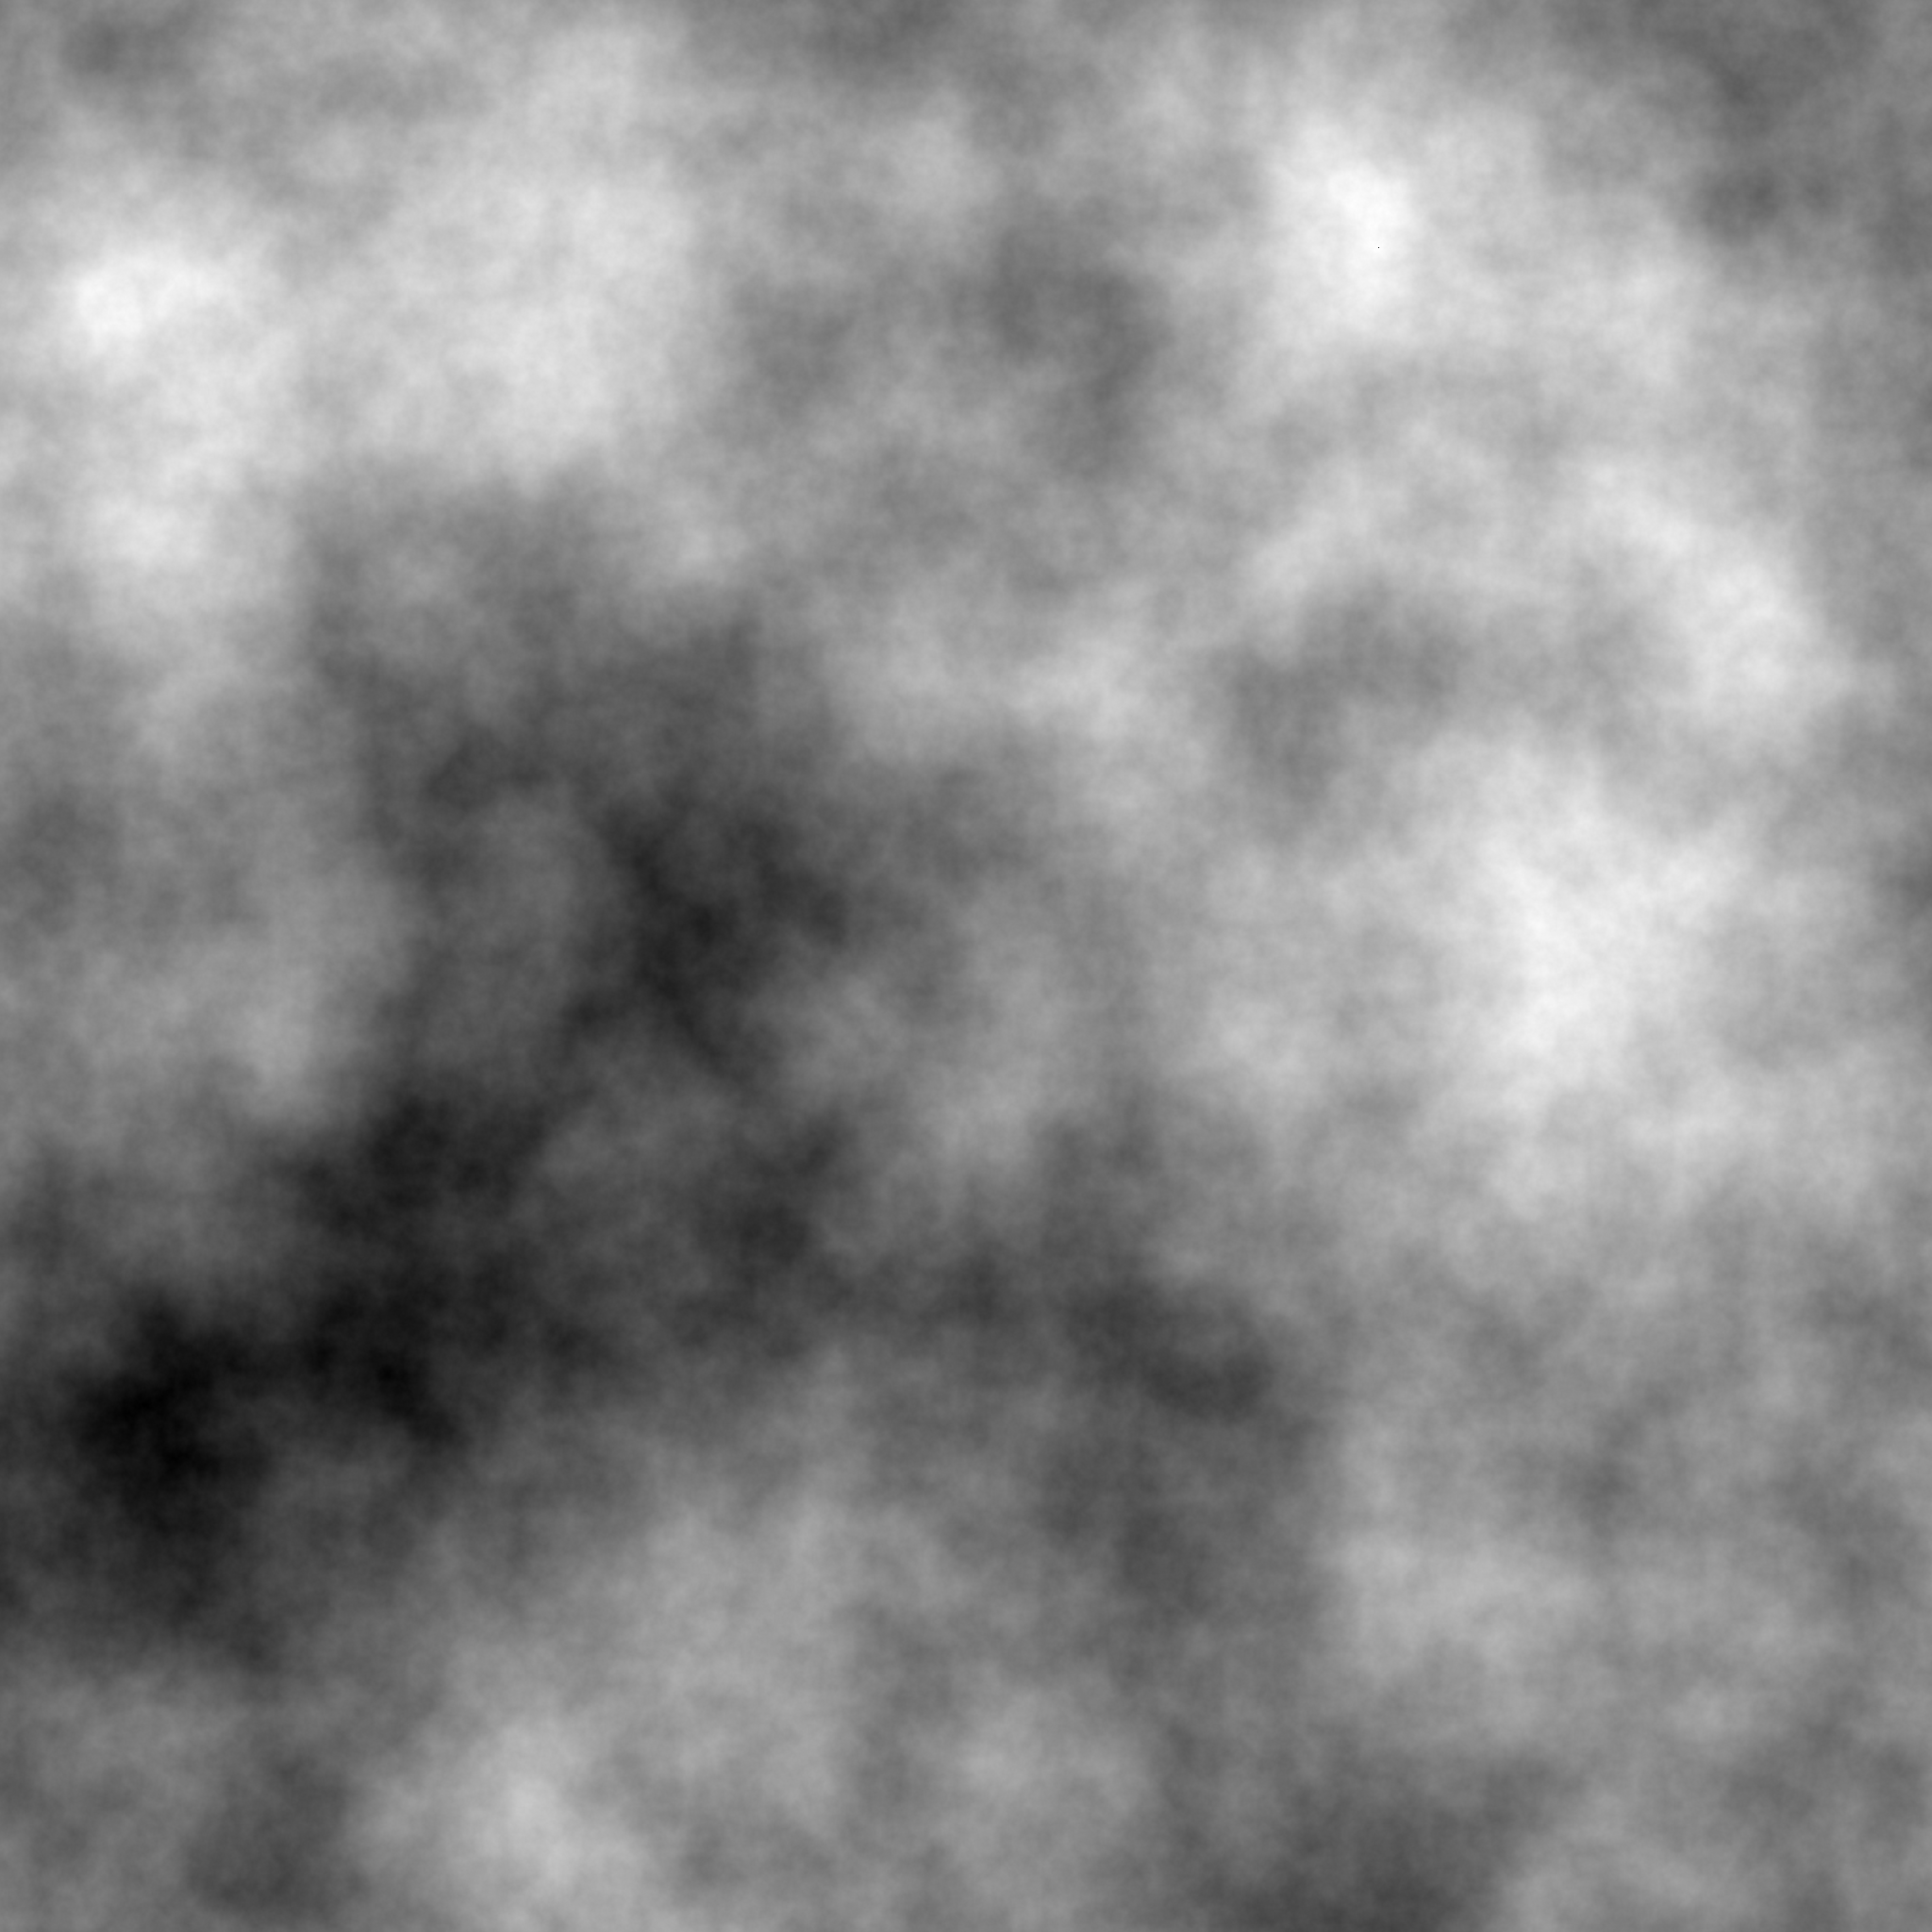
\includegraphics[width=0.4\textwidth]{data/perlin_comb_render_heightmap.png}
  \hskip 1cm
  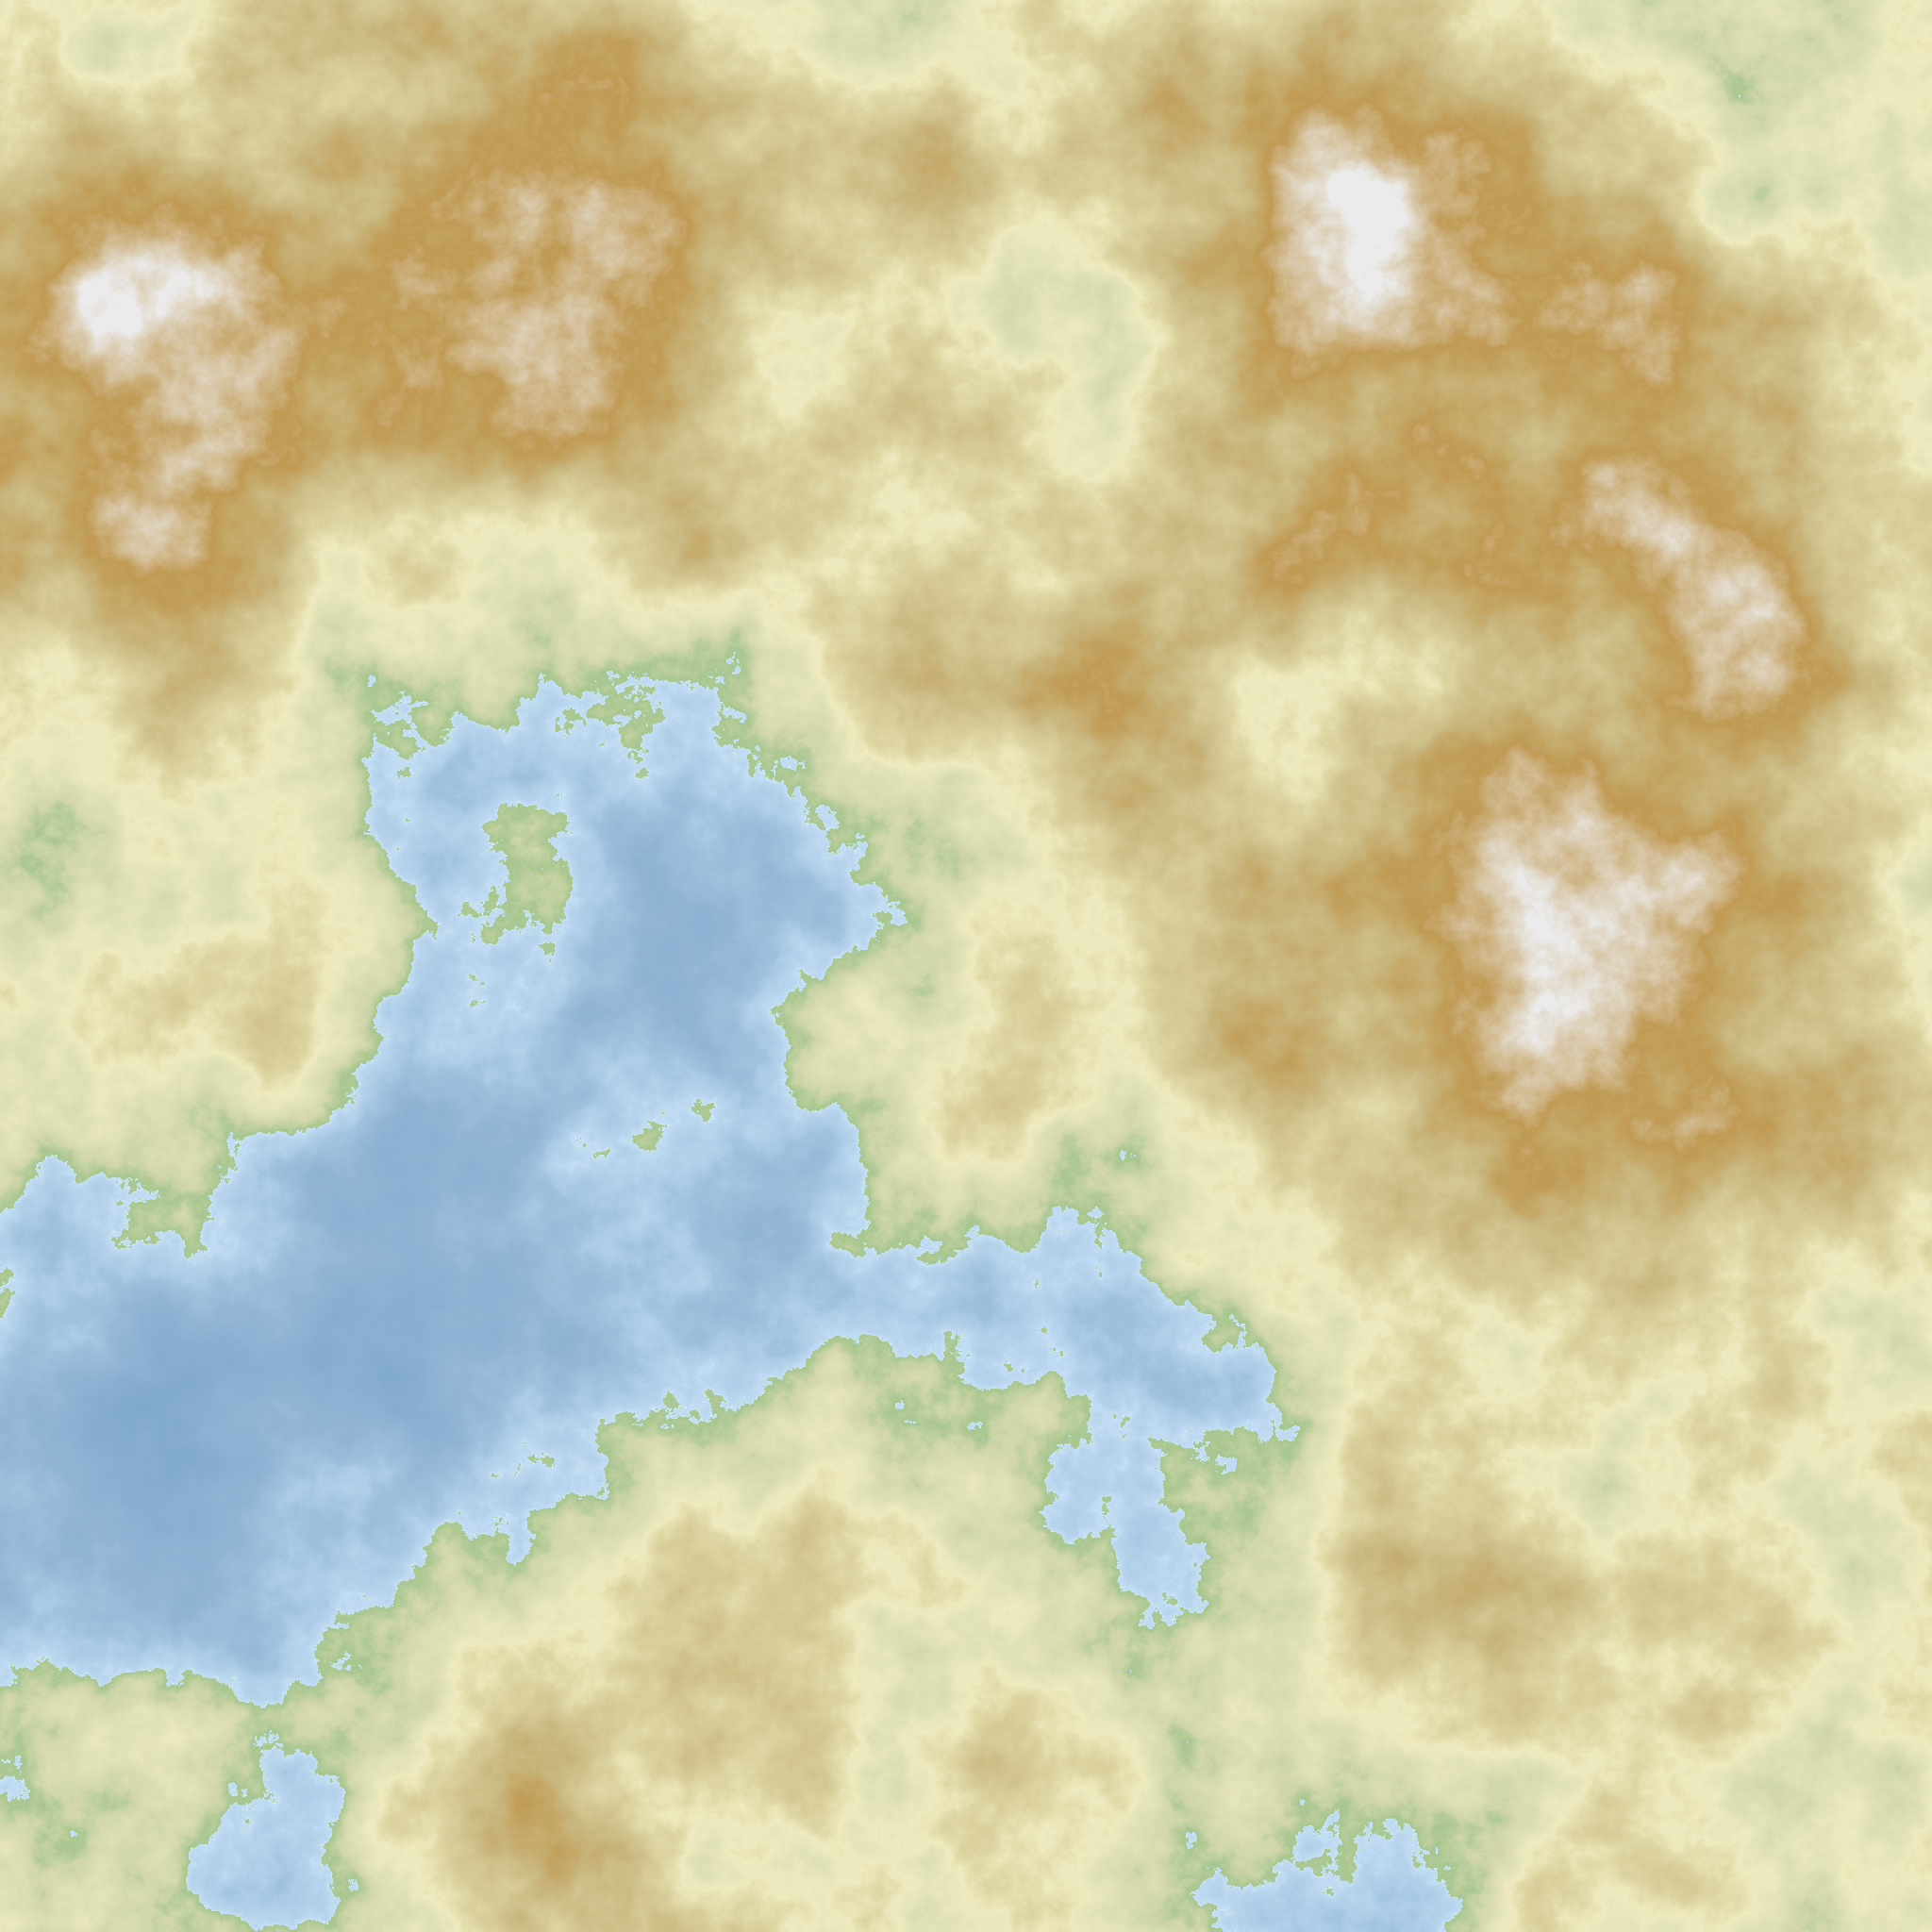
\includegraphics[width=0.4\textwidth]{data/perlin_comb_render_colored.png}
}

 
Teraz bude treba zafarbený obrázok vytieňovať. Na to použijeme jednoduchý osvetľovací model\indexItem{Alg}{Lambertov osvetľovací model}
(tzv. Lambertov). Predstav si, že máš malú plôšku, ktorá má normálový vektor $\vec n$
a nejakú základnú farbu. Čím na ňu dopadá menej svetla, tým je tmavšia. Ako viem zistiť,
koľko svetla na ňu dopadá? Ak svetlo prichádza z nejakého smeru, pozriem sa na uhol
medzi zdrojom svetla s normálovým vektorom:\\
  
\centerline{
%\tikzset{external/force remake}
%\tdplotsetmaincoords{50}{45}
%\begin{tikzpicture}[tdplot_main_coords]
\begin{tikzpicture}[x={(1,0)}, z={(0,1)}, y={(0.5,0.5)}]
  \def\dot[#1](#2){\fill[fill=#1] (#2) circle (1.2pt) ;}
  \def\sun(#1,#2,#3){
    \begin{scope}[canvas is xz plane at y=#2]
      \begin{scope}[shift={(#1,#3)},every path/.style={fill=white,draw=orange,very thick}]
        \filldraw (0,0) circle (0.2cm);
      \def\n{20}  
        \foreach \i in {0,...,\n} {
          \pgfmathsetmacro{\tmp}{\i*360/\n}
        \draw (\tmp:0.3cm) -- (\tmp:0.4cm);
        }
    \end{scope}
    \end{scope}
  }

  \def\ax{2}\def\ay{1}\def\az{2}
  \def\sx{0}\def\sy{0}\def\sz{5}
  \def\ux{1}\def\uy{4}\def\uz{0}
  \def\vx{-1}\pgfmathsetmacro{\vy}{1.0/\uy}\def\vz{0.6}

  \coordinate (Ax) at (\ax,\ay,0);
  \coordinate (h) at (0,0,\az);

  \coordinate (S) at (\sx,\sy,\sz);

  
  \normalize{\ux}{\uy}{\uz}
  \normalize{\vx}{\vy}{\vz}
  \coordinate (u) at (\ux,\uy,\uz);
  \coordinate (v) at (\vx,\vy,\vz);
  \coordinate (A) at ($(Ax)+(h)$);
  \def\s{1}
  \coordinate (P) at ($(A)-\s*(u) - \s*(v)$);
  \cross{\nx}{\ny}{\nz}{\ux}{\uy}{\uz}{\vx}{\vy}{\vz}

  \normalize{\nx}{\ny}{\nz}
  \coordinate (n) at (\nx,\ny,\nz);

  \begin{scope}[canvas is xy plane at z=0]
    \draw [gray!50, thin] (-1,-1) grid (4,4);
  \end{scope}
  \draw[orange,thick,dotted] (\sx,\sy,0)  -- (S);
  \dot[orange](\sx,\sy,0)
 
  \coordinate (u2) at (\ux,\uy,0);
  \coordinate (v2) at (\vx,\vy,0);
  \coordinate (P2) at ($(Ax)-\s*(u2)-\s*(v2)$);


  \filldraw[fill=green!10] (P) -- ($(P)+2*\s*(u)$) --($(P)+2*\s*(u)+2*\s*(v)$) -- 
  ($(P)+2*\s*(v)$) -- cycle;
  \draw[green!50!black,thick,dotted](Ax)--($(A)+(0,0,0)$);

  \coordinate (An) at ($(A)+1.5*(n)$);
  \draw[draw=none]  pic[draw, angle radius=4ex] {angle = An--A--S};

  \draw[orange,thick,->,shorten >= 3ex] (A)--node[anchor=south west]{$\vec s$}(S);
  \draw[teal,thick,->] (A)--(An) node[anchor=west]{$\vec n$};
  \dot[green!50!black](A);
  \dot[green!50!black](Ax);
  \sun(\sx,\sy,\sz)
  \node[above=1ex] at (A) {$\alpha$};

  %\drawaxes
\end{tikzpicture}}


Kosínus tohoto uhla mi vyjadruje množstvo dopadajúceho svetla: ak plôška smeruje presne na zdroj svetla, uhol je $0$,
$\cos(0)=1$, takže farba je najsilnejšia. Ako uhol rastie, $\cos(\alpha)$ postupne klesá, až keď je uhol $90^\circ$,
tak nedopadá žiadne svetlo $\cos(90^\circ)=0$.
Ak $\vec s$ je vektor smerom k svetelnému zdroju, stačí mi znormalizovať ho
a vyrátať skalárny súčin s $\vec n$ a mám $\cos(\alpha)$, ktorý potrebujem.


Posledná otvorená otázka je, ako vyrátať normálový vektor pre nejaký pixel
vo výškovej mape. Môžem to spraviť napríklad tak, že sa pozriem na 8 okolitých pixelov. Každý z nich mi dáva trojuholník,
ktorému viem vypočítať normálový vektor pomocou vektorového súčinu. Výsledný vektor potom dostanem ako priemer 
normálových vektorov trojuholníkov:\\


\centerline{
%\tikzset{external/force remake}
%\tdplotsetmaincoords{50}{45}
%\begin{tikzpicture}[tdplot_main_coords]
\begin{tikzpicture}[x={(1,0)}, z={(0,1)}, y={(0.25,0.5)}, scale=3.2]
  \def\dot[#1](#2){\fill[fill=#1] (#2) circle (0.4pt) ;}

  \begin{scope}[canvas is xy plane at z=0]
    \draw [gray!50, thin] (-0.5,-0.5) grid (2.5,2.5);
  \end{scope}

  \def\vaa{0.9}
  \def\vab{1.0}
  \def\vac{1.4}

  \def\vba{1.1}
  \def\vbb{1.2}
  \def\vbc{1.3}
  
  \def\vca{0.2}
  \def\vcb{0.6}
  \def\vcc{0.4}

  \def\chval#1{\if#10a\else\if#11b\else c\fi\fi}
  \def\w#1#2{\csname v\chval#1\chval#2\endcsname}
  \def\crd#1#2{#1,#2,\w{#1}{#2}}

  \coordinate (O) at (1,1,\w11);

  \coordinate (N) at (0,0,0);

  \foreach \i/\j/\ii/\jj/\f in {
    0/2/1/2/0%
    ,1/2/2/2/0%
    ,0/1/0/2/0%
    ,2/2/2/1/0%
    ,0/0/0/1/0%
    ,1/0/0/0/1%
    ,2/1/2/0/0%
    ,2/0/1/0/0%
  } {
    \draw[dotted] (\i,\j,0)--(\crd{\i}{\j}) (\ii,\jj,0) -- (\crd{\ii}{\jj});
    \filldraw[thin,gray,fill=yellow!10, opacity=0.6](\crd{\i}{\j})--(\crd{\ii}{\jj})--(\crd11)--cycle;

    \coordinate (A) at (\crd{\i}{\j});
    \coordinate (B) at (\crd{\ii}{\jj});
    \coordinate (P) at ($0.33*(A)+0.33*(B)+0.33*(O)$);
    \dot[blue](P)
    \pgfmathsetmacro{\ux}{\ii-1}
    \pgfmathsetmacro{\uy}{\jj-1}
    \pgfmathsetmacro{\uz}{\w{\ii}{\jj}-\w11}
    \pgfmathsetmacro{\vx}{\i-1}
    \pgfmathsetmacro{\vy}{\j-1}
    \pgfmathsetmacro{\vz}{\w{\i}{\j}-\w11}
    \cross{\nx}{\ny}{\nz}{\ux}{\uy}{\uz}{\vx}{\vy}{\vz}
    \normalize{\nx}{\ny}{\nz}
    \typeout{(\ux,\uy,\uz) x (\vx,\vy,\vz) =(nrm) (\nx,\ny,\nz)}
    \coordinate (n) at (\nx,\ny,\nz);
    \draw[blue,->](P)--($(P)+0.3*(n)$);
    \coordinate (N) at ($(N)+(n)$);
    \if\f1
      \draw[thick,red,->](O)--node[anchor=east]{$\vec u$}(A);
      \draw[thick,magenta,->](O)--node[anchor=north west, pos=0.6]{$\vec v$}(B);
    \fi
  }
  \coordinate (O) at (\crd11);
  \draw[thick,teal,->] (O) -- ($(O)+0.125*(N)$) node[above]{$\vec n$};

  \foreach \i in {0,1,2}{
    \foreach \j in {0,1,2} {
      \dot[black](\crd{\i}{\j})
    }}

    
  \draw[gray,brace=0.1ex/mirror] (0,0,0)--node[below=1.2ex]{$s$}(1,0,0);

  %\drawaxes
\end{tikzpicture}}


Naprogramovať sa to dá napríklad takto:


\begin{lstlisting}
Vec3 normala(Tabulka<double> &H, int i, int j, double s = 1) {
  Vec3 res;
  vector<Vec> dir{{0, 1},   {1, 1},  {1, 0},  {1, -1}, {0, -1},
                  {-1, -1}, {-1, 0}, {-1, 1}, {0, 1}};
  for (int t = 0; t < dir.size() - 1; t++) {
    int i0 = i + dir[t].x,     j0 = j + dir[t].y, 
        i1 = i + dir[t + 1].x, j1 = j + dir[t + 1].y;
    res +=
        -1.0 *
        (
         (Vec3{s * dir[t].x, s * dir[t].y, H(i0, j0)} 
          - Vec3{0, 0, H(i, j)}) 
          ^ // vektorový súčin
         (Vec3{s * dir[t + 1].x, s * dir[t + 1].y, H(i1, j1)} -
          Vec3{0, 0, H(i, j)})
        );
  }
  return res.normalize();
}
\end{lstlisting}


Táto funkcia dostane ako parameter tabuľku \vb{H} a pozíciu pixela \vb{i,j}.
Navyše dostanem parameter \vb{s}, ktorý hovorí, ako ďaleko sú od seba jednotlivé pixely
(t.j. výškovú mapu si predstavujem ako sieť s krokom \vb{s}).


Pre obrázok s rozmermi $2048\times2048$ som si nastavil smer svetla na 
\prg!Vec3 light{-1, 1, 12};! a \prg!double s=0.004;! a 
z výškovej mapy \vb{H} som si vyrátal tabuľku \prg!Tabulka<double> N!
takto:

\begin{lstlisting}
light.normalize();
for (int i = 0; i < H.m; i++)
  for (int j = 0; j < H.n; j++)
    if (H(i, j) <= wl)
      N(i, j) = 1;
    else
      N(i, j) = light * normala(H, i, j, s);
\end{lstlisting}


Výsledok je na obrázku vľavo. Obrázok vpravo vznikol tak, že som každú farbu pixela na ofarbenej mape
prenásobil koeficientom\footnote{%
t.j. zobral som $60\%$ pôvodnej farby a $40\%$ som rozdelil od čiernej po pôvodnú farbu
podľa normály. Nie je to úplne ideálne, ale môže nám to postačiť.
}  \prg!0.6 + 0.4 * max(0.0, N(i, j));!\\


\centerline{
  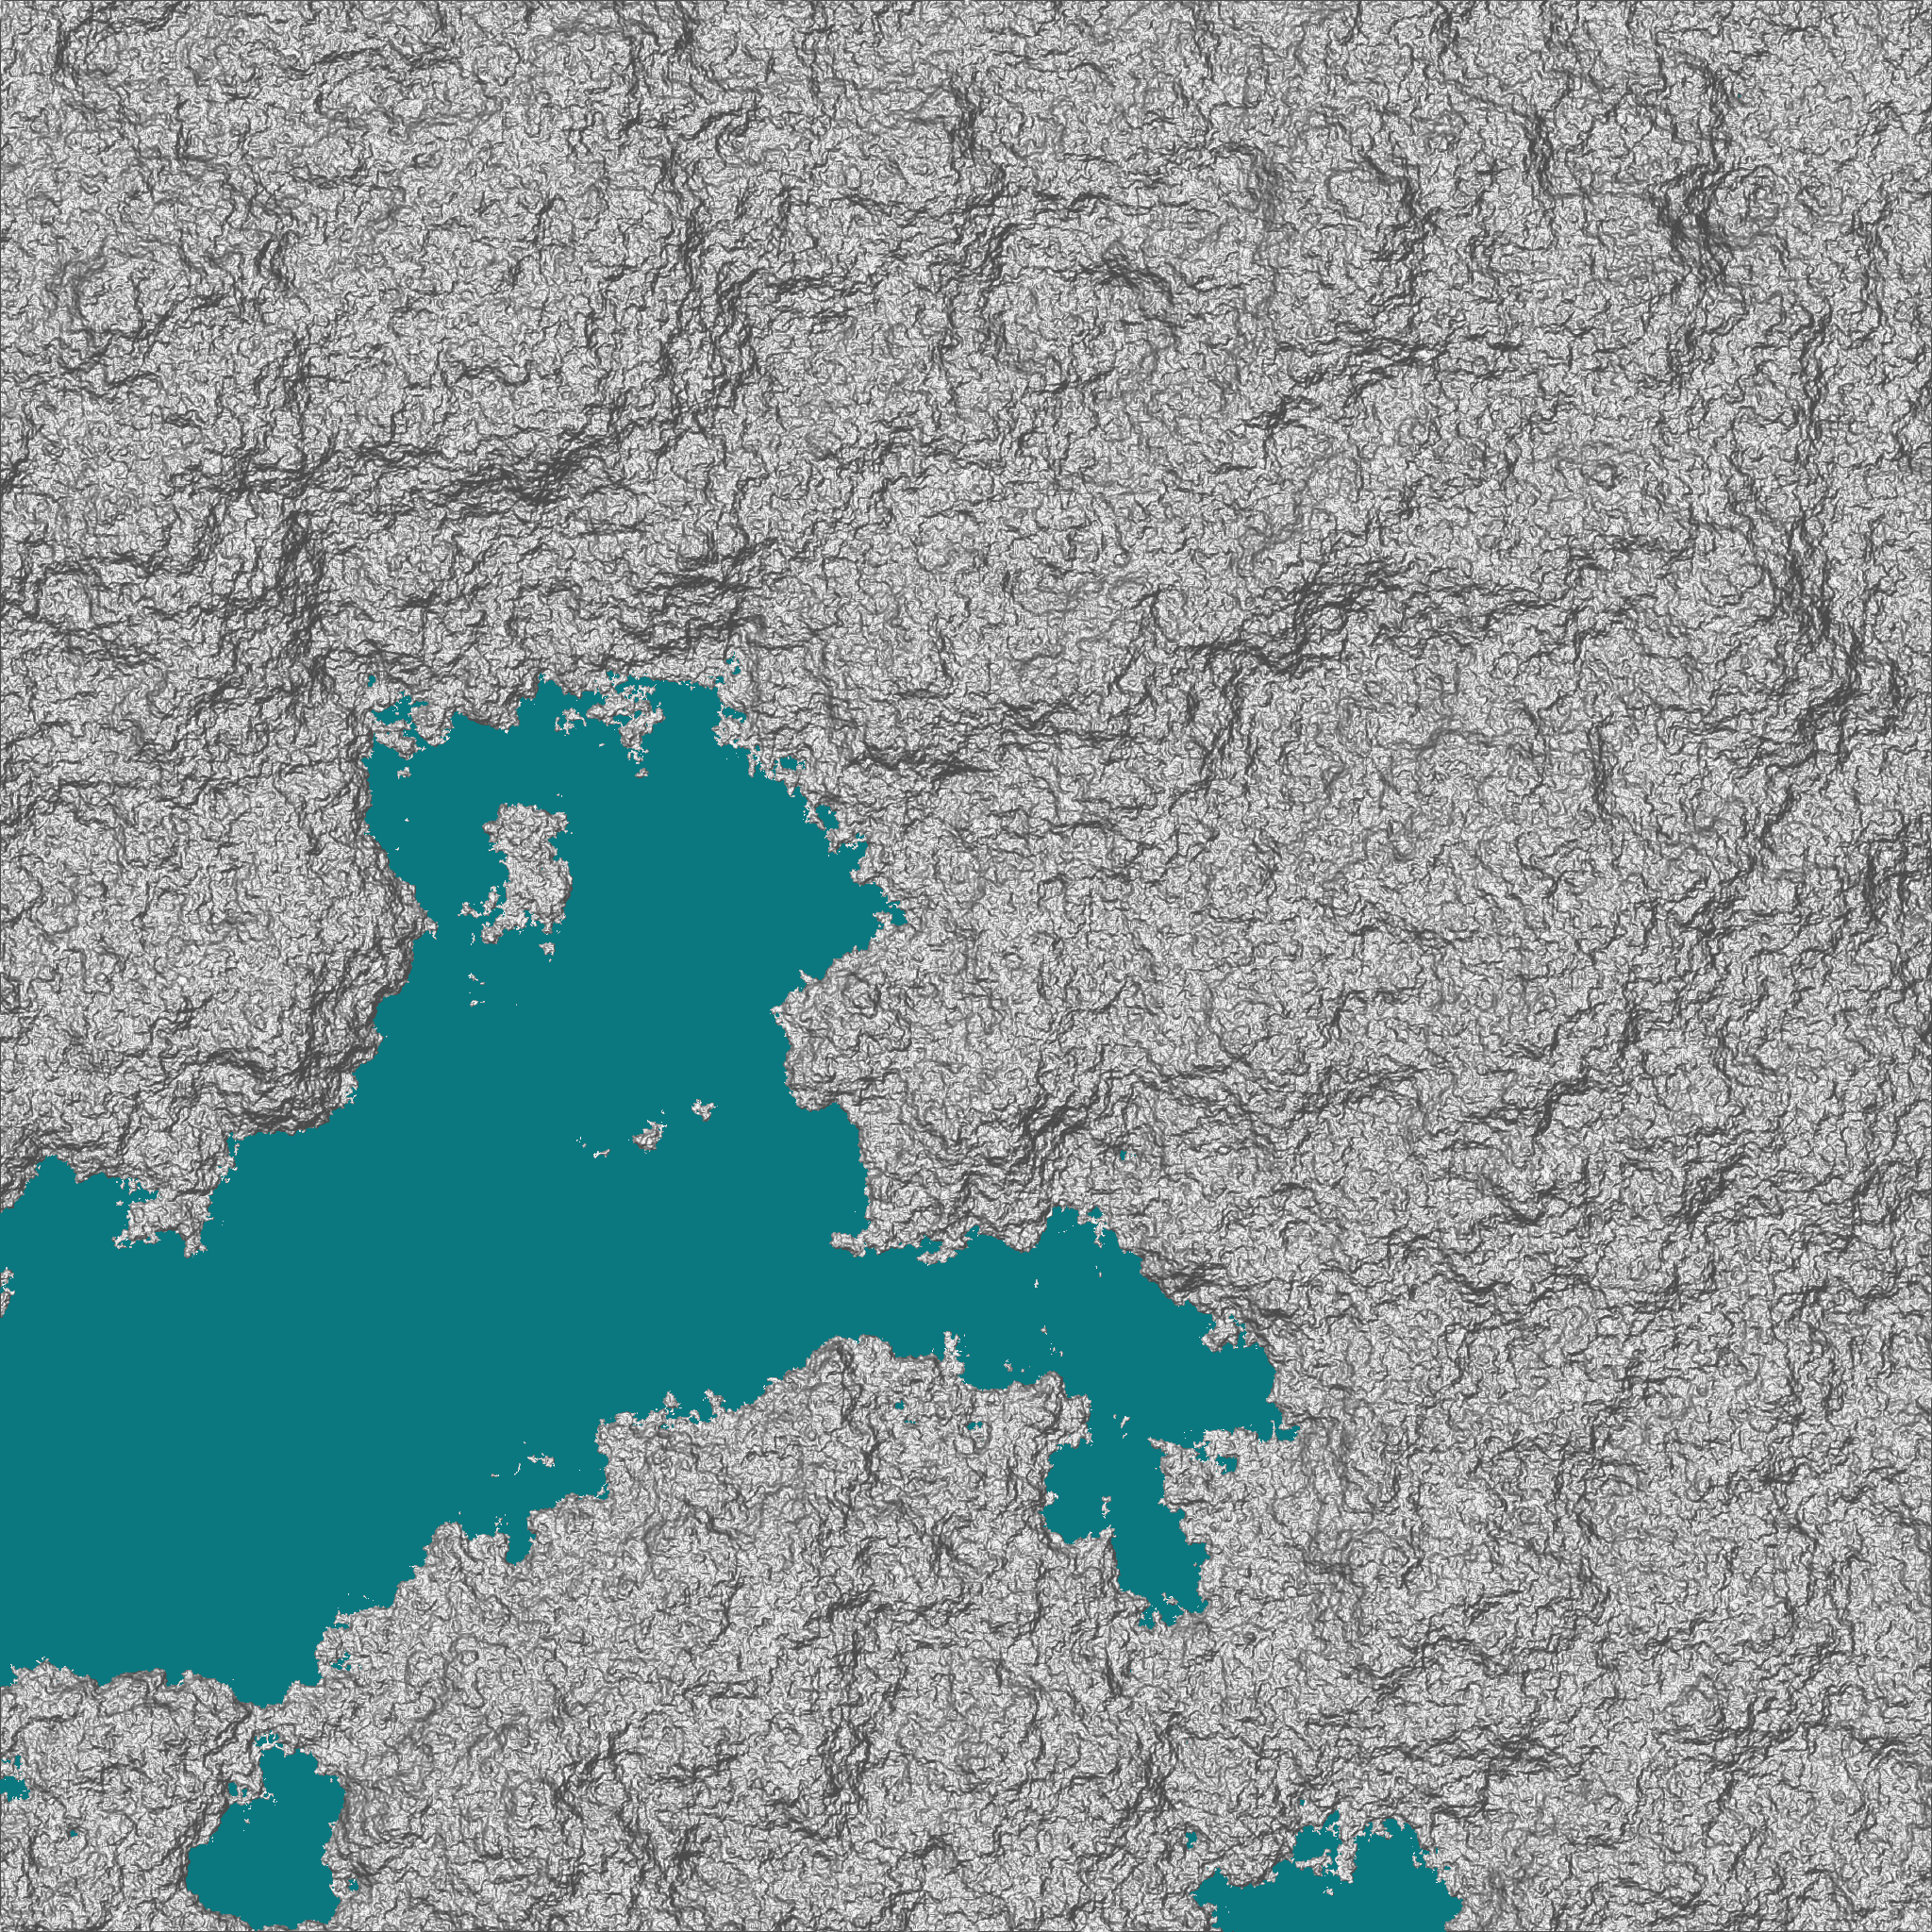
\includegraphics[width=0.4\textwidth]{data/perlin_comb_render_normal.png}
  \hskip 1cm
  \includegraphics[width=0.4\textwidth]{data/perlin_comb_render_rendered.png}
}


Toto už vyzerá ako mapa terénu, aj keď zrovna ostrov to nie je. To sa dá ale ľahko napraviť pri generovaní
výškovej mapy: okrem Perlinovho šumu sa navyše každý bod posunie dole úmerne jeho vzdialenosti od stredu 
obrázka. Okraje klesnú a v strede ostane ostrov. S trochou hrania sa s klesaním okrajov
a zvýraznením hôr som dospel k takémuto
výsledku:\\


\centerline{
  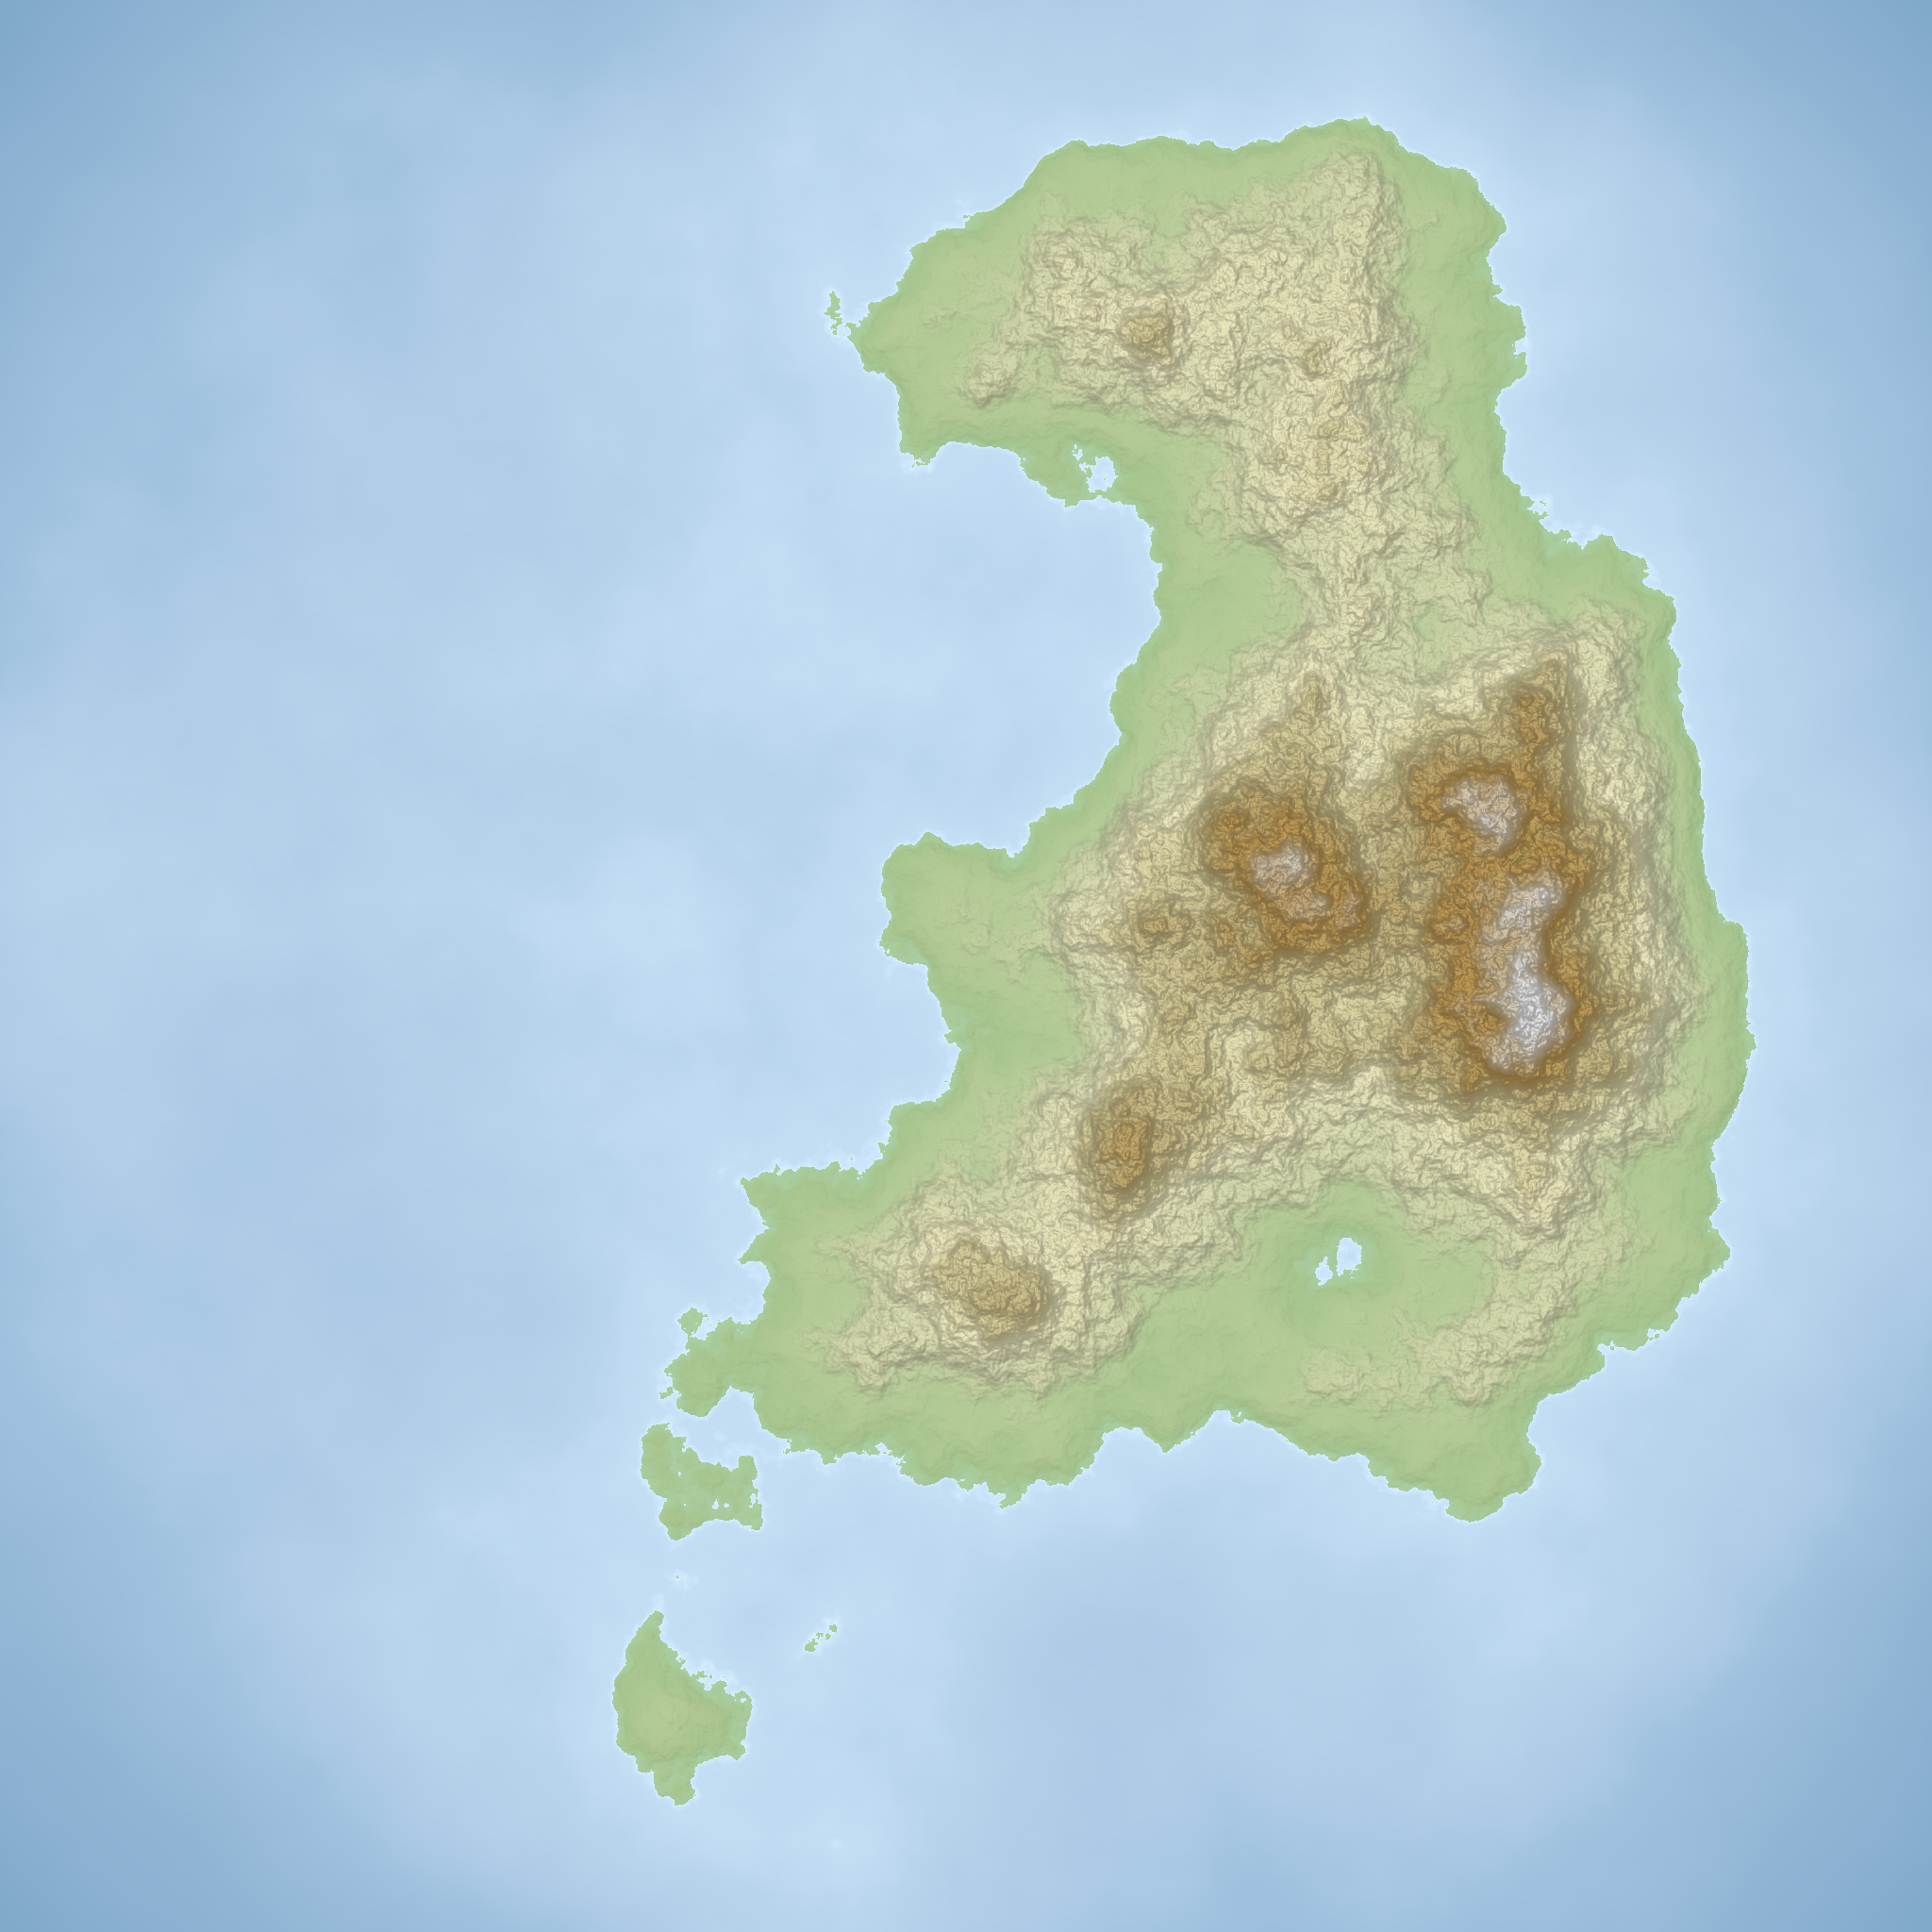
\includegraphics[width=0.7\textwidth]{data/86_rendered_dry.png}
}


Úplne posledná vec, ktorá tomu chýba, sú doliny riek a fjordy. Rozhodol som sa preto spraviť jednoduchú\indexItem{Alg}{simulácia erózie}
fyzikálnu simuláciu vodnej erózie. Urobiť realistickú virtuálnu eróziu je téma sama osebe, ale 
v \link%
{https://www.firespark.de/resources/downloads/implementation\%20of\%20a\%20methode\%20for\%20hydraulic\%20erosion.pdf}%
{bakalárskej práci Hansa Beyera}
je veľmi zjednodušený a ľahko naprogramovateľný prístup, ktorý si tu môžeme vyskúšať.
Hlavná idea je, že na povrch našej výškovej mapy budeme púšťať kvapky\footnote{
  Vzhľadom na mierku, ktorú máme, to bude skôr ako futbalový štadión plný vody, ale
  volajme to kvapka.}. Kvapka má nejaký objem vody a v nej je rozpustený nejaký objem 
bahna. Ak je bahna málo a kvapka ide rýchlo, vymyje kúsok z povrchu: výšková mapa sa trochu 
zníží a v kvapke bude viac bahna. Naopak, ak je bahna veľa a kvapka ide pomaly, bahno sa bude
usadzovať: v kvapke ho ostane menej a povrch sa trochu zvýši.
Ako zistíme, ktorým smerom sa bude kvapka pohybovať? Krátka odpoveď je, že v smere, ktorým
ukazuje normálový vektor. Dalo by sa to pomerne jednoducho spočítať, ale nateraz sa uspokojme
s intuitívnou predstavou podľa obrázka




\centerline{
%\tikzset{external/force remake}
%\tdplotsetmaincoords{50}{45}
%\begin{tikzpicture}[tdplot_main_coords]
\begin{tikzpicture}[x={(1,0)}, z={(0,1)}, y={(0.5,0.5)}]
%\begin{tikzpicture}[x={(1,0)}, z={(0,0)}, y={(0,1)}]
  \def\dot[#1](#2){\fill[fill=#1] (#2) circle (1.2pt) ;}

  \def\rotplane[#1][#2][#3]{ %zxz
  \begin{scope}[canvas is xy plane at z=0]
    \draw [gray!20, very thin] (-1.5,-1.5) grid (1.5,1.5);
  \end{scope}
    \def\h{1}
    \def\d{1}
    \pgfmathsetmacro{\ax}{-0.5*\d}\pgfmathsetmacro{\ay}{-0.5*\d}\pgfmathsetmacro{\az}{0}
    \pgfmathsetmacro{\bx}{0.5*\d}\pgfmathsetmacro{\by}{-0.5*\d}\pgfmathsetmacro{\bz}{0}
    \pgfmathsetmacro{\cx}{0.5*\d}\pgfmathsetmacro{\cy}{0.5*\d}\pgfmathsetmacro{\cz}{0}
    \pgfmathsetmacro{\dx}{-0.5*\d}\pgfmathsetmacro{\dy}{.5*\d}\pgfmathsetmacro{\dz}{0}
    \pgfmathsetmacro{\nx}{0}\pgfmathsetmacro{\ny}{0}\pgfmathsetmacro{\nz}{1}

    \rotz[#1]{\ax}{\ay}{\az}
    \rotz[#1]{\bx}{\by}{\bz}
    \rotz[#1]{\cx}{\cy}{\cz}
    \rotz[#1]{\dx}{\dy}{\dz}
    \rotz[#1]{\nx}{\ny}{\nz}

    \rotx[#2]{\ax}{\ay}{\az}
    \rotx[#2]{\bx}{\by}{\bz}
    \rotx[#2]{\cx}{\cy}{\cz}
    \rotx[#2]{\dx}{\dy}{\dz}
    \rotx[#2]{\nx}{\ny}{\nz}

    \rotz[#3]{\ax}{\ay}{\az}
    \rotz[#3]{\bx}{\by}{\bz}
    \rotz[#3]{\cx}{\cy}{\cz}
    \rotz[#3]{\dx}{\dy}{\dz}
    \rotz[#3]{\nx}{\ny}{\nz}

    \begin{scope}[shift={(0,0,\h)}]
      \filldraw[fill=teal!20, opacity=0.6]  (\ax,\ay,\az) -- (\bx,\by,\bz) -- (\cx,\cy,\cz) -- (\dx,\dy,\dz) -- cycle;
    \draw[->] (0,0,0) -- (\nx,\ny,\nz);
    \dot[black](0,0,0);
    \end{scope}

    \draw[dashed] (0,0,0) -- (0,0,\h);
    \draw[->,magenta] (0,0,0) -- (\nx,\ny,0);

  }


  \rotplane[0][45][0]
  \begin{scope}[shift={(2,0)}]
    \rotplane[0][45][90]
  \end{scope}
  \begin{scope}[shift={(4,0)}]
    \rotplane[30][40][60]
  \end{scope}
  \begin{scope}[shift={(6,0)}]
    \rotplane[210][320][45]
  \end{scope}


  %\drawaxes
\end{tikzpicture}}


\phantomsection\label{page:gradient}
Predstav si malú plôšku, z ktorej trčí normálový vektor ako klinec. Ktorým smerom klincom
pohneš, tým smerom sa plôška nakloní, a tade bude aj kvapka padať. Takže stačí nám
zrátať normálový vektor v 3D a pozrieť sa na jeho priemet, t.j. na zložky v smere $x$
a $y$. Výsledný 2D vektor sa volá {\em gradient} a udáva smer, ktorým plôška klesá. 


Pre účely simulácie si budeme pozíciu kvapky pamätať v reálnych číslach ako
premennú \prg!Vec pos!. Výšková mapa mi bude udávať výšku v bodoch s celočíselnými
súradnicami (tieto budem volať {\em mrežové body}).
Pre danú pozíciu si skutočnú výšku vyrátame bilineárnou interpoláciou zo 
štyroch susedných mrežových bodov. Normálu vyrátam podobne -- najprv vyrátam normálové 
vektory v štyroch susedných mrežových bodoch a výsledok zrátam bilineárnou interpoláciou.\\



\centerline{
%\tikzset{external/force remake}
\begin{tikzpicture}[x={(1,0)}, z={(0,0.7)}, y={(0.25,0.5)}, scale=4]
%\begin{tikzpicture}[x={(1,0)}, z={(0,0)}, y={(0,1)}, scale=3.5]
  \def\dot[#1](#2){\fill[fill=#1] (#2) circle (0.4pt) ;}

  \begin{scope}[canvas is xy plane at z=0]
    \draw [gray!50, thin] (-0.2,-0.2) grid (1.2,1.2);
  \end{scope}

  \def\vs{0.5}
  \def\newv(#1)#2#3#4{
    \def\tmpx{#2}
    \def\tmpy{#3}
    \def\tmpz{#4}
    \normalize{\tmpx}{\tmpy}{\tmpz}
    \coordinate (#1) at (\vs*\tmpx,\vs*\tmpy,\vs*\tmpz);
    \coordinate (#1!0) at (\vs*\tmpx,\vs*\tmpy,0);
  }
  \def\chval#1{\if#10a\else\if#11b\else\if#12c\else d\fi\fi\fi}
  \def\w#1#2{\csname v\chval#1\chval#2\endcsname}
  \def\crd#1#2{#1,#2,\w{#1}{#2}}

  \def\vaa{1.0} \newv(n00){-0.2}{-0.3}{1}
  \def\vab{1.3} \newv(n01){-0.2}{-0.7}{1.5}

  \def\vba{0.8} \newv(n10){-0.2}{-0.3}{1}
  \def\vbb{1.5} \newv(n11){-0.2}{-0.7}{1} 
  
  \foreach \i in {0,1}{
    \foreach \j in {0,1} {
      \coordinate (A\i\j) at (\crd{\i}{\j});
      \coordinate (A\i\j!0) at (\i,\j,0);
    }}


  \def\px{0.5} \def\py{0.7}


  \coordinate (P!0) at (\px,\py,0);
  \coordinate (P0!0) at (\px,0,0);
  \coordinate (P1!0) at (\px,1,0);

  \coordinate (P0) at ($(A00)!\px!(A10)$);
  \coordinate (P1) at ($(A01)!\px!(A11)$);
  \coordinate (P) at ($(P0)!\py!(P1)$);

  \foreach \a in {0,1}{
  \coordinate (nP\a) at ($(n0\a)!\px!(n1\a)$);
  \coordinate (nP\a!0) at ($(n0\a!0)!\px!(n1\a!0)$);
  }
  \coordinate (nP) at ($(nP0)!\py!(nP1)$);
  \coordinate (nP!0) at ($(nP0!0)!\py!(nP1!0)$);

  \filldraw[fill=yellow!10, opacity=0.3] (A00) -- (A10) -- (A11) -- (A01) -- cycle;

  \draw[thin,dashed,gray] (P) -- (P!0);

  \foreach \a in {0,1}{
  \draw[magenta,->] (P\a)--($(P\a)+(nP\a)$);
  \draw[magenta!30,->](P\a!0)--($(P\a!0)+(nP\a!0)$);
  }
  \draw[magenta, dotted] (P0)--(P1);
  \draw[magenta!30, dotted] (P0!0)--(P1!0);
  \draw[magenta,thick, ->] (P)--($(P)+(nP)$) node[above] {\vb{norm}};
  \draw[magenta,thick,->](P!0)--($(P!0)+(nP!0)$) node[anchor = north east]  {\vb{g}};

  %\draw let \p1=(nP0!0),\p2=(n00!0),\p3=(n10!0) in (2,0) node{\x1,\y1 :: \x2,\y2 :: \x3,\y3};
  




  \foreach \i in {0,1}{
    \foreach \j in {0,1} {
      \draw[teal,->] (A\i\j) -- ($(A\i\j)+(n\i\j)$);
      \draw[cyan,->] (A\i\j!0) -- ($(A\i\j!0)+(n\i\j!0)$);

      \dot[black](A\i\j)
      \draw[dashed,gray,thin] (A\i\j!0) -- (A\i\j);
    }}

    \dot[black](P!0);
    \node[anchor=north west] at (P!0) {\vb{pos}};
    
  \foreach \p in {P,A00!0,A11!0} {
  \dot[black](\p)
  }

  \node[anchor=north west] at (P) {\vb{vyska(pos)}};


  \node[anchor = south east] at (A00!0) {\vb{(ix, iy)}};   
  \node[anchor = north west ] at (A11!0) {\vb{(ix + 1, iy + 1)}};   

  %\drawaxes
\end{tikzpicture}}



Simulácia jednej kvapky bude vyzerať takto. Kvapka sa na začiatku zajví na náhodnej pozícii

\begin{lstlisting}
Vec pos{dis(rnd) * n, dis(rnd) * n};
\end{lstlisting}

Budeme simulovať niekoľko krokov, na
to budeme mať konštantu \vb{lifetime}. V každom kroku vyrátame gradient \prg!Vec g;!
tak, ako sme to práve opísali. Nový smer kvapky \prg!dir! získame tak, že interpolujeme
gradient a predchádzajúci smer s parametrom \vb{zotrvacnost}, t.j. budeme robiť
\prg!dir = lerp(g, dir, zotrvacnost);!. Výsledný smer normalizujeme tak, aby sa 
kvapka pohla o vzdialenosť jedna. 
Vyrátame pôvodnú výšku a novú výšku a 
ich rozdiel označíme \vb{delta}.


O kvapke si navyše pamätáme rýchlosť\footnote{%
  Rýchlosť používam iba pri výpočte erózie. Pri určovaní smeru sa vždy pohnem o jednotku.
  To je kvôli tomu, aby rýchle kvapky nepreskakovali mrežové body a pomalé kvapky sa zbytočne
  nesimulovali veľakrát na tom istom mieste.},
  objem vody (číslo od 0 do 1) a množstvo rozpusteného bahna.
 Koľko bahna sa z kvapky môže usadiť závisí od sklonu, rýchlosti a množstva vody:

 
 \centerline{
   \prg!double dasausadit =  max(-delta, min_sklon) * rychlost * voda * rozpustnost;!} 


Pričom \prg!min_sklon! a \prg!rozpustnost! sú konštanty, ktoré si na začiatku nejak nastavíme.
Teraz môžu nastať dva prípady: ak kvapka tečie dokopca, alebo nesie viac bahna, ako 
\prg!dasauasdit!, bahno sa bude usádzať. Ak tečie dokopca (t.j. $\vb{delta}>0$)
bahno sa snaží vyplniť rozdiel výšok, t.j. usadí sa \prg!min(delta, bahno)!. V opačnom
prípade sa usadí \prg!(bahno - dasausadit) * usadzanie;!, kde \vb{usadzanie} je opäť
ďalší parameter z rozsahu 0 až 1. 
Usadené bahno odrátame z bahna v kvapke a prirátame ho k výškovej mape.
Pri tom použijeme zase bilineárnu interpoláciu, t.j. ak množstvo usadeného mahna máme 
v premennej \vb{usadit}, 
tak do výškovej mapy \vb{H} rozdelíme usadeninu 
podľa pozície kvapky medzi meržovými bodmi tak,
že bližšie mrežové body dostanú viac a vzdialenejšie menej\footnote{
Nasledovný program je možno trochu neprehľadný, ale vyskúšaj si, čo znamená pre konkrétne 
mrežové body. Napr. pre \vb{dx=0}, \vb{dy=0} vyplynie, že \vb{H(ix,iy)}
dostane časť \vb{(1 - p.x) * (1 - p.y)}. Ak napr. \vb{p} je na pozícii \vb{(ix,iy)},
tak \vb{p.x} aj \vb{p.y} je 0 a všetok materiál ide do \vb{H(ix,iy)}. Ak by 
\vb{pos} bolo na opačnom konci na pozícii \vb{(ix+1, iy+1)}, tak do \vb{H(ix,iy)}
nejde nič. 
}:


\vbox{
\begin{lstlisting}
int ix = pos.x, iy = pos.y;     // mrežový bod po zaokrúhlení pozície
Vec p{pos.x - ix, pos.y - iy};  // pozícia v rámci gridu

for (int dx = 0; dx < 2; dx++)
  for (int dy = 0; dy < 2; dy++) {
    H(ix + dx, iy + dy) += usadit * (dx * p.x + (1 - dx) * (1 - p.x)) *
                           (dy * p.y + (1 - dy) * (1 - p.y));
  }
\end{lstlisting}
}


Ak sa bahno neusádza, tak nastáva erózia: časť materiálu z výškovej mapy sa presunie
do kvapky. Aká veľká časť sa uberie, kontroluje ďalší parameter \vb{erozia}.
Materiál budeme uberať nielen zo susedných mrežových bodov, ale
zo širšieho okolia, aby nevznikali príilš úzke a strmé kaňony:

\begin{lstlisting}
double urvat = min((dasausadit - bahno) * erozia, -delta);

// odoberie zo širšieho okolia podľa toho, ako sú nastavené váhy
for (int dx = 0; dx < 2 * r + 1; dx++)
  for (int dy = 0; dy < 2 * r + 1; dy++) {
    int i = ix - r + dx, j = iy - r + dy;
    double kusok = urvat * vahy[dx][dy];
    H(i, j) -= kusok;
    bahno += kusok;
  }
\end{lstlisting}



Pole \vb{vahy} bude ako ''štetec'' rozmerov $2\vb{r}+1\times2\vb{r}+1$, ktorý 
si doredu pripravíme tak, aby pokrýval okolie do vzdialenosti \vb{r}, 
v strede mal väčšie hodnoty ako na krajoch a dokopy mal súčet 1 takto (číslo 
v políčku je váha v percentách):\\



\centerline{\begin{tikzpicture}[scale=0.7]
  \def\r{4}
  
  \pgfmathtruncatemacro{\n}{2*\r}
  \foreach \dx [
    remember=\suma (initially 0),    
  ]in {0,...,\n}{
    \foreach\dy[
      remember=\sumb (initially \suma),
    ] in {0,...,\n}{
      \pgfmathsetmacro{\dist}{sqrt((\r-\dx)*(\r-\dx)+(\r-\dy)*(\r-\dy))/(\r+1)}
       \ifdim\dist pt<1.0pt\pgfmathsetmacro{\w}{1-\dist}\else\pgfmathsetmacro{\w}{0}\fi
       \pgfmathsetmacro{\sumb}{\sumb+\w}
       \xdef\suma{\sumb}
    }
    \xdef\pako{\suma}
  }

  \foreach \dx in {0,...,\n} {
    \foreach \dy in {0,...,\n} {
      \pgfmathsetmacro{\dist}{sqrt((\r-\dx)*(\r-\dx)+(\r-\dy)*(\r-\dy))/(\r+1)}
       \ifdim\dist pt<1.0pt\pgfmathsetmacro{\w}{1-\dist}\else\pgfmathsetmacro{\w}{0}\fi
       \pgfmathsetmacro{\tmp}{100*\w/\pako}
       \pgfmathtruncatemacro{\c}{\tmp/6*90}
       \fill[teal!\c](\dx,\dy) rectangle ++(1,1);
       \ifnum\c<50\def\c{100}\else\def\c{0}\fi
       \ifdim\tmp pt>0pt\node[black!\c] at (0.5+\dx,0.5+\dy) {{\scriptsize 
         \calc[precision=1]{\tmp}}};\fi
     }
   }

  \draw[teal] (0,0) grid (\n+1,\n+1);
\end{tikzpicture}}


To sa dá naprogramovať napr. takto:


\begin{lstlisting}
double sum = 0;
for (int dx = 0; dx < 2 * r + 1; dx++)
  for (int dy = 0; dy < 2 * r + 1; dy++) {
    // vzdialenosť od stredu
    double dist = sqrt((r - dx) * (r - dx) + (r - dy) * (r - dy)) / (r + 1);
    double w = 0;
    if (dist < 1) w = (1 - dist);
    vahy[dx][dy] = w;
    sum += w;
  }
for (int dx = 0; dx < 2 * r + 1; dx++)
  for (int dy = 0; dy < 2 * r + 1; dy++) vahy[dx][dy] /= sum;
\end{lstlisting}


Pozícia \prg![r][r]! je  presne v strede poľa, preto 
$\sqrt{(\vb{r}-\vb{dx})^2+(\vb{r}-\vb{dy})^2}$ je vzdialenosť políčka 
\prg![dx][dy]! od stredu. Vzdialenosť predelíme \vb{r + 1}, aby sme dostali kruh s 
polomerom 1. Pozície mimo kruhu budú mať hodnotu 0, pozície v kruhu hodnotu 
úmernú vzdialenosti od stredu. Nakoniec každú hodnotu vydelíme súčtom\footnote{
  To je typická finta ako zaručiť, že celkový súčet je 1. Ak mám čísla
  $a_1, a_2,\ldots a_n$ a označím $s=a_1+a_2+\cdots+a_n$, tak keď zoberiem čísla
  $b_1=\frac{a_1}{s}$, $b_2=\frac{a_2}{s}$, \ldots, $b_n=\frac{a_n}{s}$, tak 
  ich vzájomné relatívne veľkosti sa nezmenia, lebo som všetky vydelil rovnakým číslom,
  a ich súčet bude $b_1+\cdots+b_n=\frac{a_1}{s}+\cdots+\frac{a_n}{s}=
  \frac{1}{s}(a_1+\cdots+a_n)=\frac{s}{s}=1$.
}.


Nakoniec upravíme rýchlosť podľa fyzikou inšpirovaného vzťahu

\begin{lstlisting}
if (delta < 0) delta *= -1;
rychlost = sqrt(rychlost * rychlost + delta * gravitacia);
\end{lstlisting}

kde \vb{gravitacia} je parameter, a odparíme časť vody 
\prg!voda *= (1 - odparovanie)! kde \vb{odparovanie} je ešte iný parameter.

\begin{uloha}
  Naprogramuj triedu \vb{Eroder}, ktorá v konštruktore dostane referenciu na 
  výškovú mapu a má funkciu \vb{kvap}, ktorá na nej odsimuluje jednu kvapku.
\end{uloha}

Výhodou tejto metódy je, že je jednoduchá, nevýhodou je, že má strašne veľa parametrov,
ktoré treba správne nastaviť, ak má výsledok vyzerať dobre\footnote{
  V pôvodnej práci je ešte jedno odporúčanie: keďže pri úpravách výškovej mapy sú zmeny
  pri jednej kvapke veľmi malé, kvôli reprezentácii reálnych čísel môže prísť
  k podtečeniu: číslo, ktoré prirátavame je tak malé, že sa v mantise neprejaví.
  Preto je lepšie udržovať
  si zmeny v separátnej tabuľke a až nakoniec ich prirátať k výškovej mape.}.


Po troche hrania sa s parametrami som dostal výsledok, s ktorým som bol viac-menej spokoný.
Na obrázku vľavo sú dráhy kvapiek, vpravo je ostrov po erózii.\\


\centerline{
  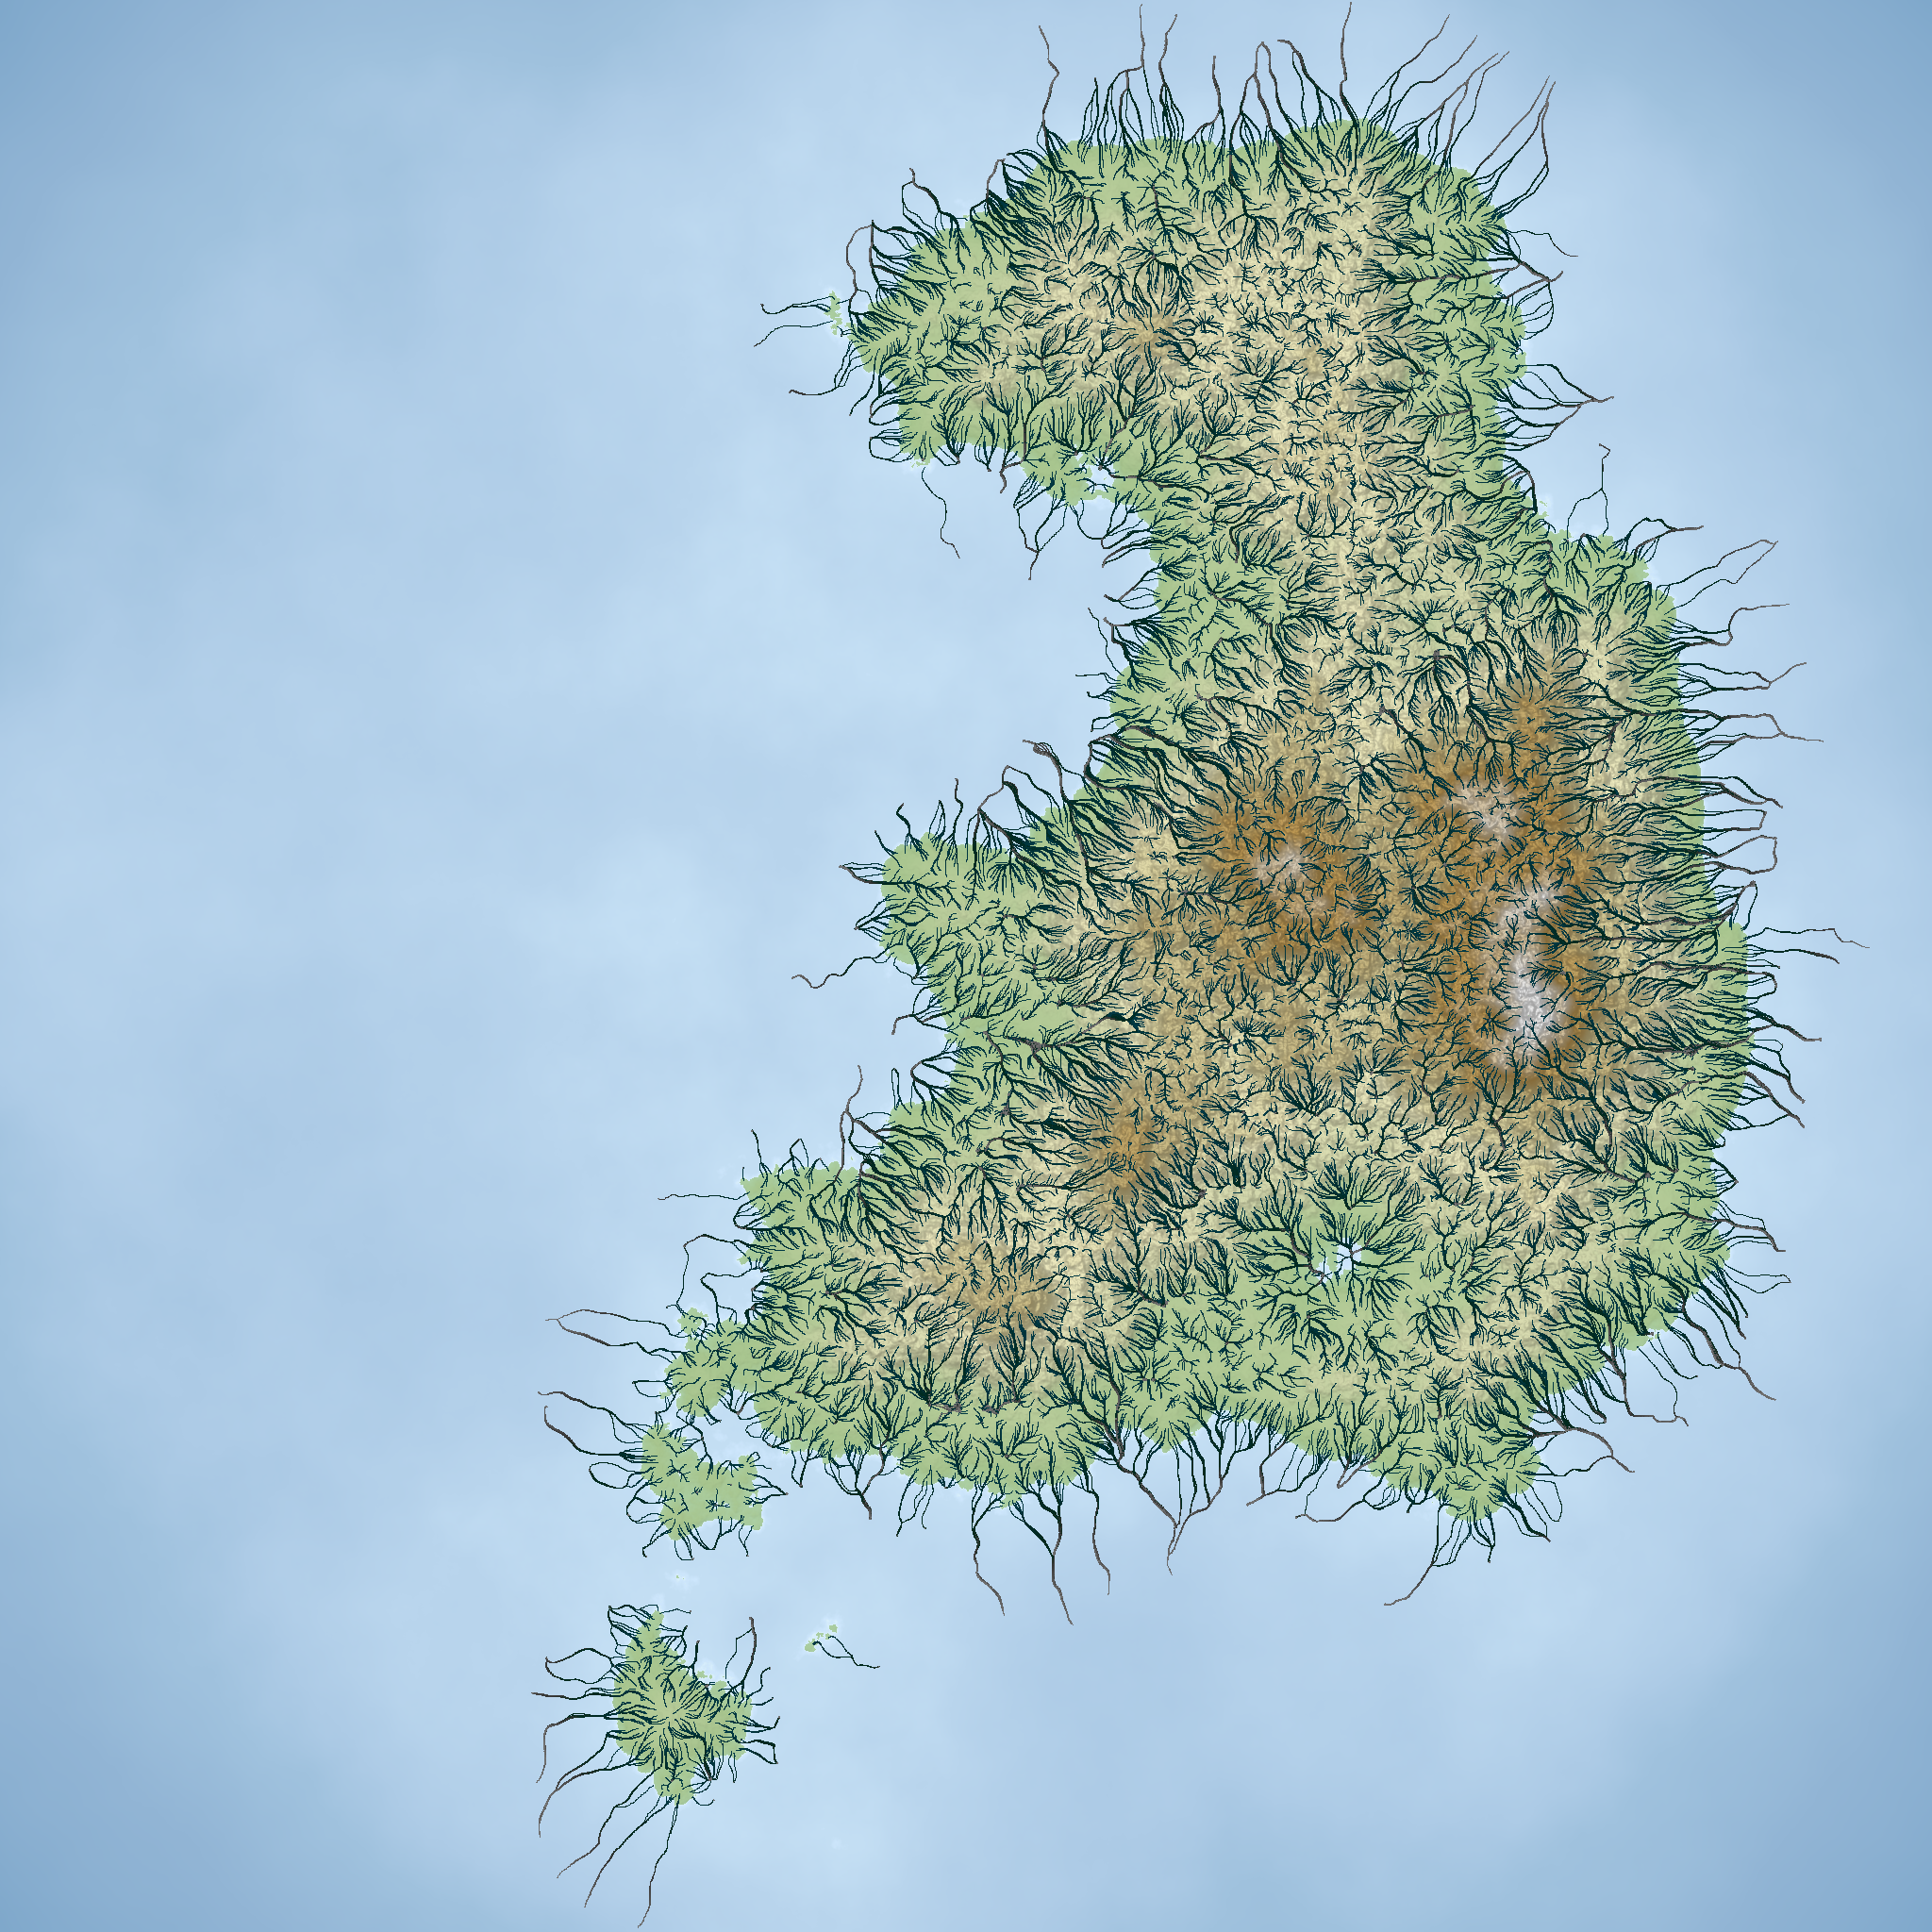
\includegraphics[width=0.45\textwidth]{data/86_rendered_droplets.png}
  \hfill
  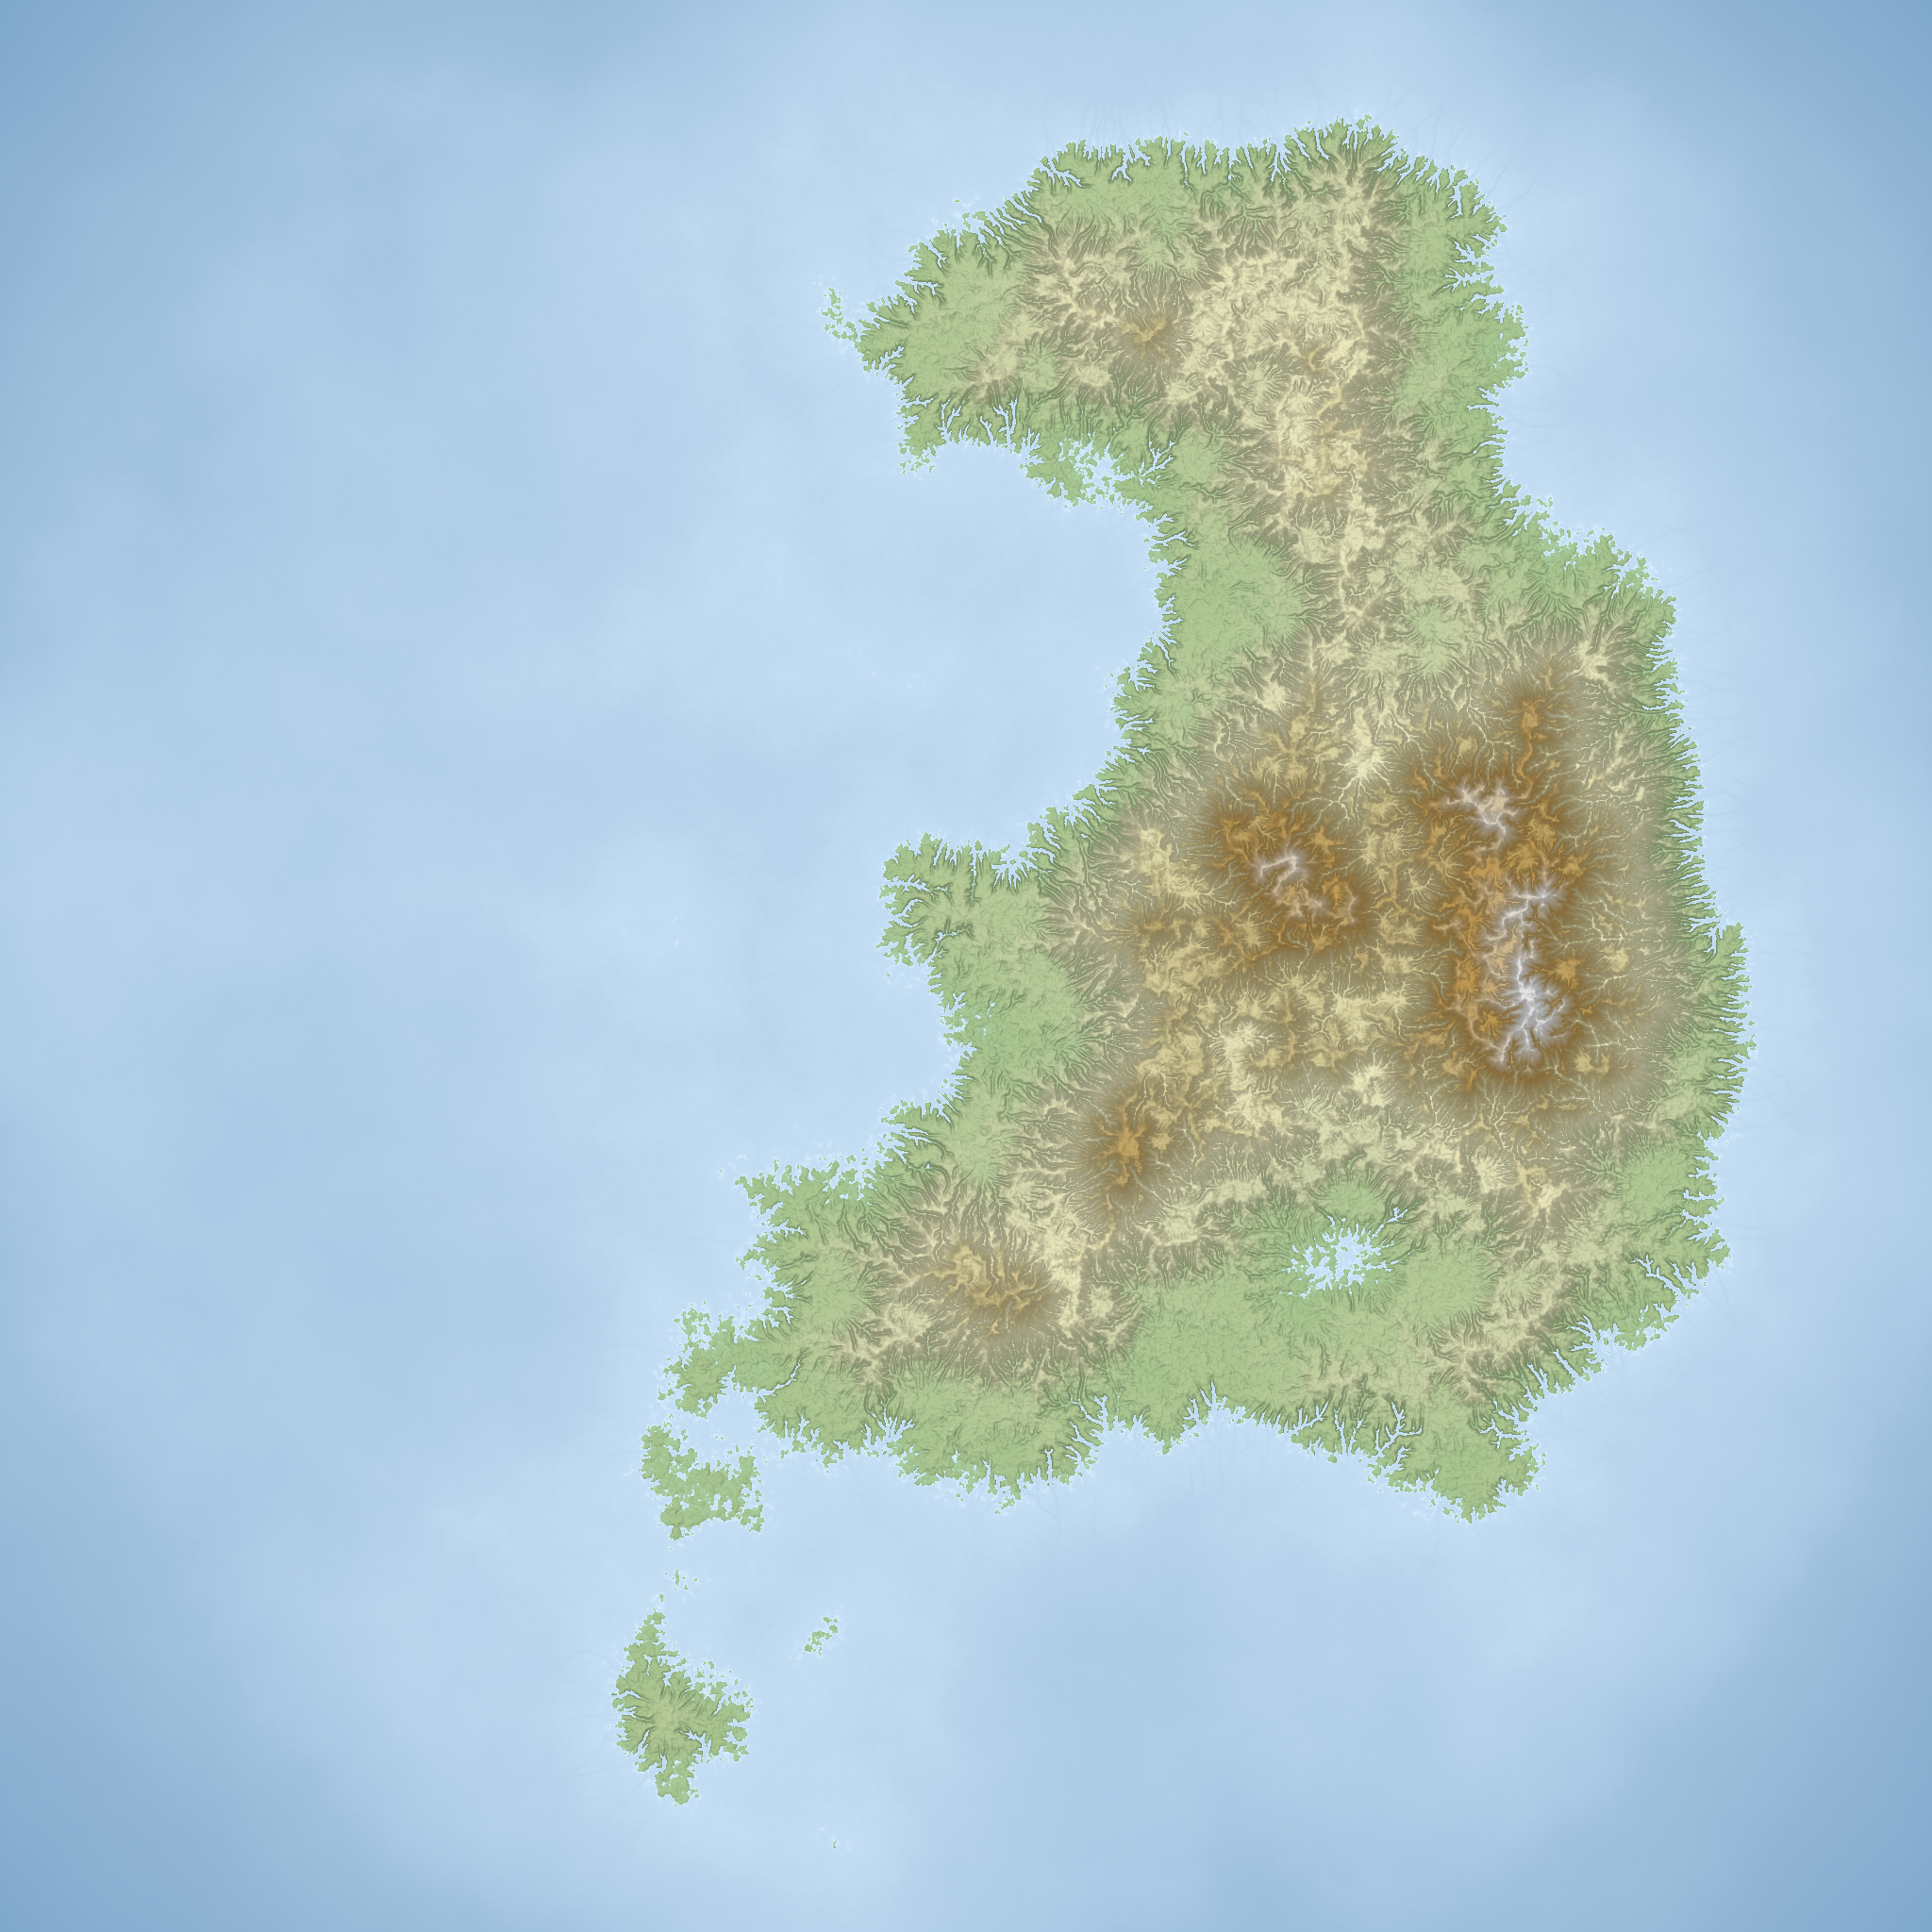
\includegraphics[width=0.45\textwidth]{data/86_rendered.png}
}

\def\ulohaTarget{Dir}
\begin{uloha}
  Daj to celé dokopy a naprogramuj generovanie náhodných ostrovov.
\end{uloha}
\def\ulohaTarget{File}

Tu je niekoľko ďalších ostrovov, ktoré sa vygenerovali s rôznymi seedmi:

\def\tmp#1{
  \centerline{
\foreach\n in {#1}{
  \includegraphics[width=0.33\textwidth]{data/ostrovy/\n_rendered.png}
}}}

\tmp{100,263,264}

\vskip 1ex

\tmp{265,266,267}

\vskip 1ex

\tmp{26,273,53}


Samozrejme, v tomto projekte by sa dalo pokračovať k realistickejším výsledkom, ale chcel
som ti len ukázať, ako sa náhodné čísla dajú použiť na vytváranie vecí, ktoré sú 
''len trochu'' náhodné. 

